%% This is an example first chapter.  You should put chapter/appendix that you
%% write into a separate file, and add a line \include{yourfilename} to
%% main.tex, where `yourfilename.tex' is the name of the chapter/appendix file.
%% You can process specific files by typing their names in at the 
%% \files=
%% prompt when you run the file main.tex through LaTeX.
\chapter{Results and Testing}
This chapter will describe the results of my work using an excerpt of of W. A. Mozart's \textit{Eine kleine Nachtmusik, K.525} as an example. It will also use an excerpt of W. A. Mozart's \textit{String Quartet No.7 in E-flat major, K.160/159a} as an example where K.525 doesn't fit the specifications. This chapter will also look at timing metrics of the system.

\section{Example 1: Eine kleine Nachtmusik, K.525, W. A. Mozart)}		`
This section will go through an example of how the entire \texttt{OMRMIDICorrector} system works on W. A. Mozart's \textit{Eine kleine Nachtmusik, K.525}.

\begin{figure}[H]
\centering
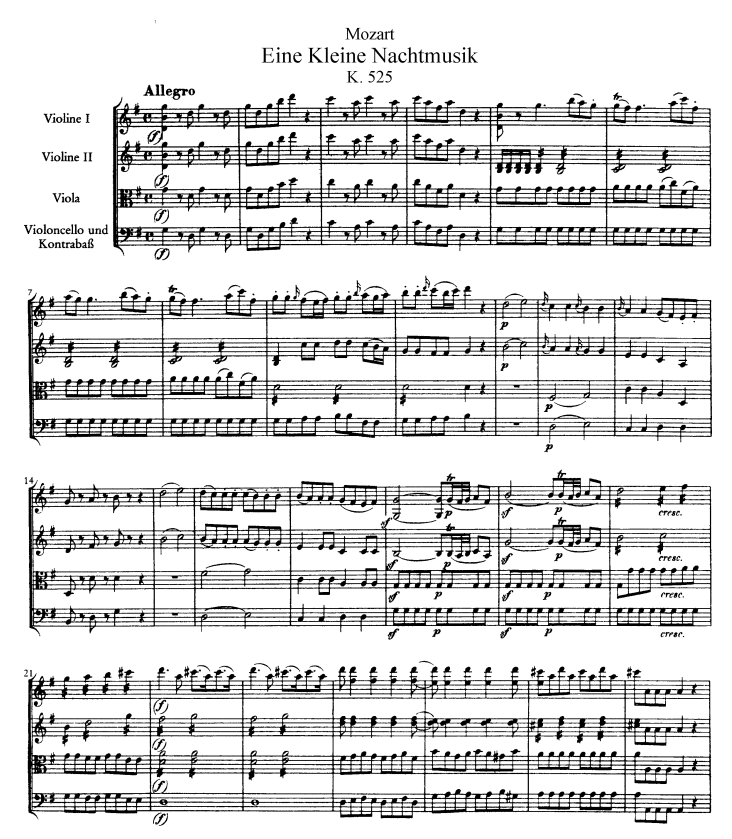
\includegraphics[width =.9\textwidth]{k525originalomrscan}
\caption{The first page of the scanned copy of the score found on IMSLP.}
\end{figure}

\subsection{Musical Properties of K.525}
I chose K.525 as the example piece for many of it music properties that make it a difficult but interesting piece to align. 

\subsubsection{Bass and Cello Doubling}
In the original scanned score, there are only four parts because the bass part doubles the cello part one octave lower. However, in the MIDI encoding, there must be five separate voices. Thus, in the preprocessing step of the \texttt{OMRMiDICorrector}, it would be ideal for the system to recognize this. Otherwise, in instances where the \texttt{OMRMIDIC```orrector} could not pair up the parts between the input OMR stream and the input MIDI stream, there would be an error thrown, and alignment and correction would not happen. 

\subsubsection{Tremolos}
Starting in measure 5 in the original scanned score, the second violin has tremolo notes, instead of repeated \nth{16} notes written out. The OMR parser in SmartScore is not robust enough to recognize the slashes across the stem of the note as tremolo markings and instead interprets it as a single note. The MIDI protocol has no way of indicating tremolos, so the second violin's notes in measure 5 are encoded as regular \nth{16} notes. Ideally, the aligner would be robust enough to align tremolo measures with non-tremolo measures even though there will be a huge discrepancy in the number of notes present in the measure.

\subsection{Preparing the Raw Input}
The basic raw input of the system is an OMR score and a MIDI file. A scanned copy of the score was found in IMSLP \cite{k525}, the source for much free public domain sheet music. The MIDI file was sourced from the Yale MIDI Archive. 

I used SmartScore's built-in OMR tool to convert the scanned score of K.525 into an ENF file. Then I exported the post-OMR file as a musicXML file.

Similarly for the K.525 MIDI file, I used SmartScore to parse the original file and exported it as a musicXML file. 

The last step of preparing the raw input is to parsing the musicXML files with the \texttt{music21} library so that they are \texttt{Stream} objects. This can be done by passing in the musicXML filepaths to the \texttt{parse} method in the \texttt{converter} class. We will call these two parsed streams \texttt{k525midiStream} and \texttt{k525omrStream}. 
\begin{minted}{python}
from music21 import *
k525MidiFilepath = "pathto/k525/miditoxml.xml"
k525OmrFilepath= "pathto/k525/omrtoxml.xml"
k525midistream = converter.parse(k525MidiFilepath)
k525omrstream = converter.parse(k525OmrFilepath)
\end{minted}
\subsection{Running \texttt{OMRMIDICorrector} on K.525}
After the raw input has been massaged into \texttt{Stream} objects, the aligning process is simple. We create an instance of an \texttt{OMRMIDICorrector} object with the two streams as parameters. For the purposes of this example, we will use the default hasher that is built into the \texttt{OMRMIDICorrector} class. We will set the \texttt{debugShow} to \texttt{True} so that we can visualize the alignment between pairwise streams. Finally, we will call \texttt{processRunner} which will hash and align the parts in the stream. For now, we will manually create the \texttt{Fixer} objects for stream fixing. The aligner is able to correctly identify that the repeated \nth{16} notes 

\begin{minted}{python}
from music21 import *
OMC = alpha.analysis.omrMidiCorrector
k525omc = OMC.OMRMIDICorrector(k525midistream, k525omrstream)
k525omc.debugShow = True
k525omc.processRunner()
\end{minted}

These are the outputs of the \texttt{showChanges} function.

\begin{figure}[H]
\centering
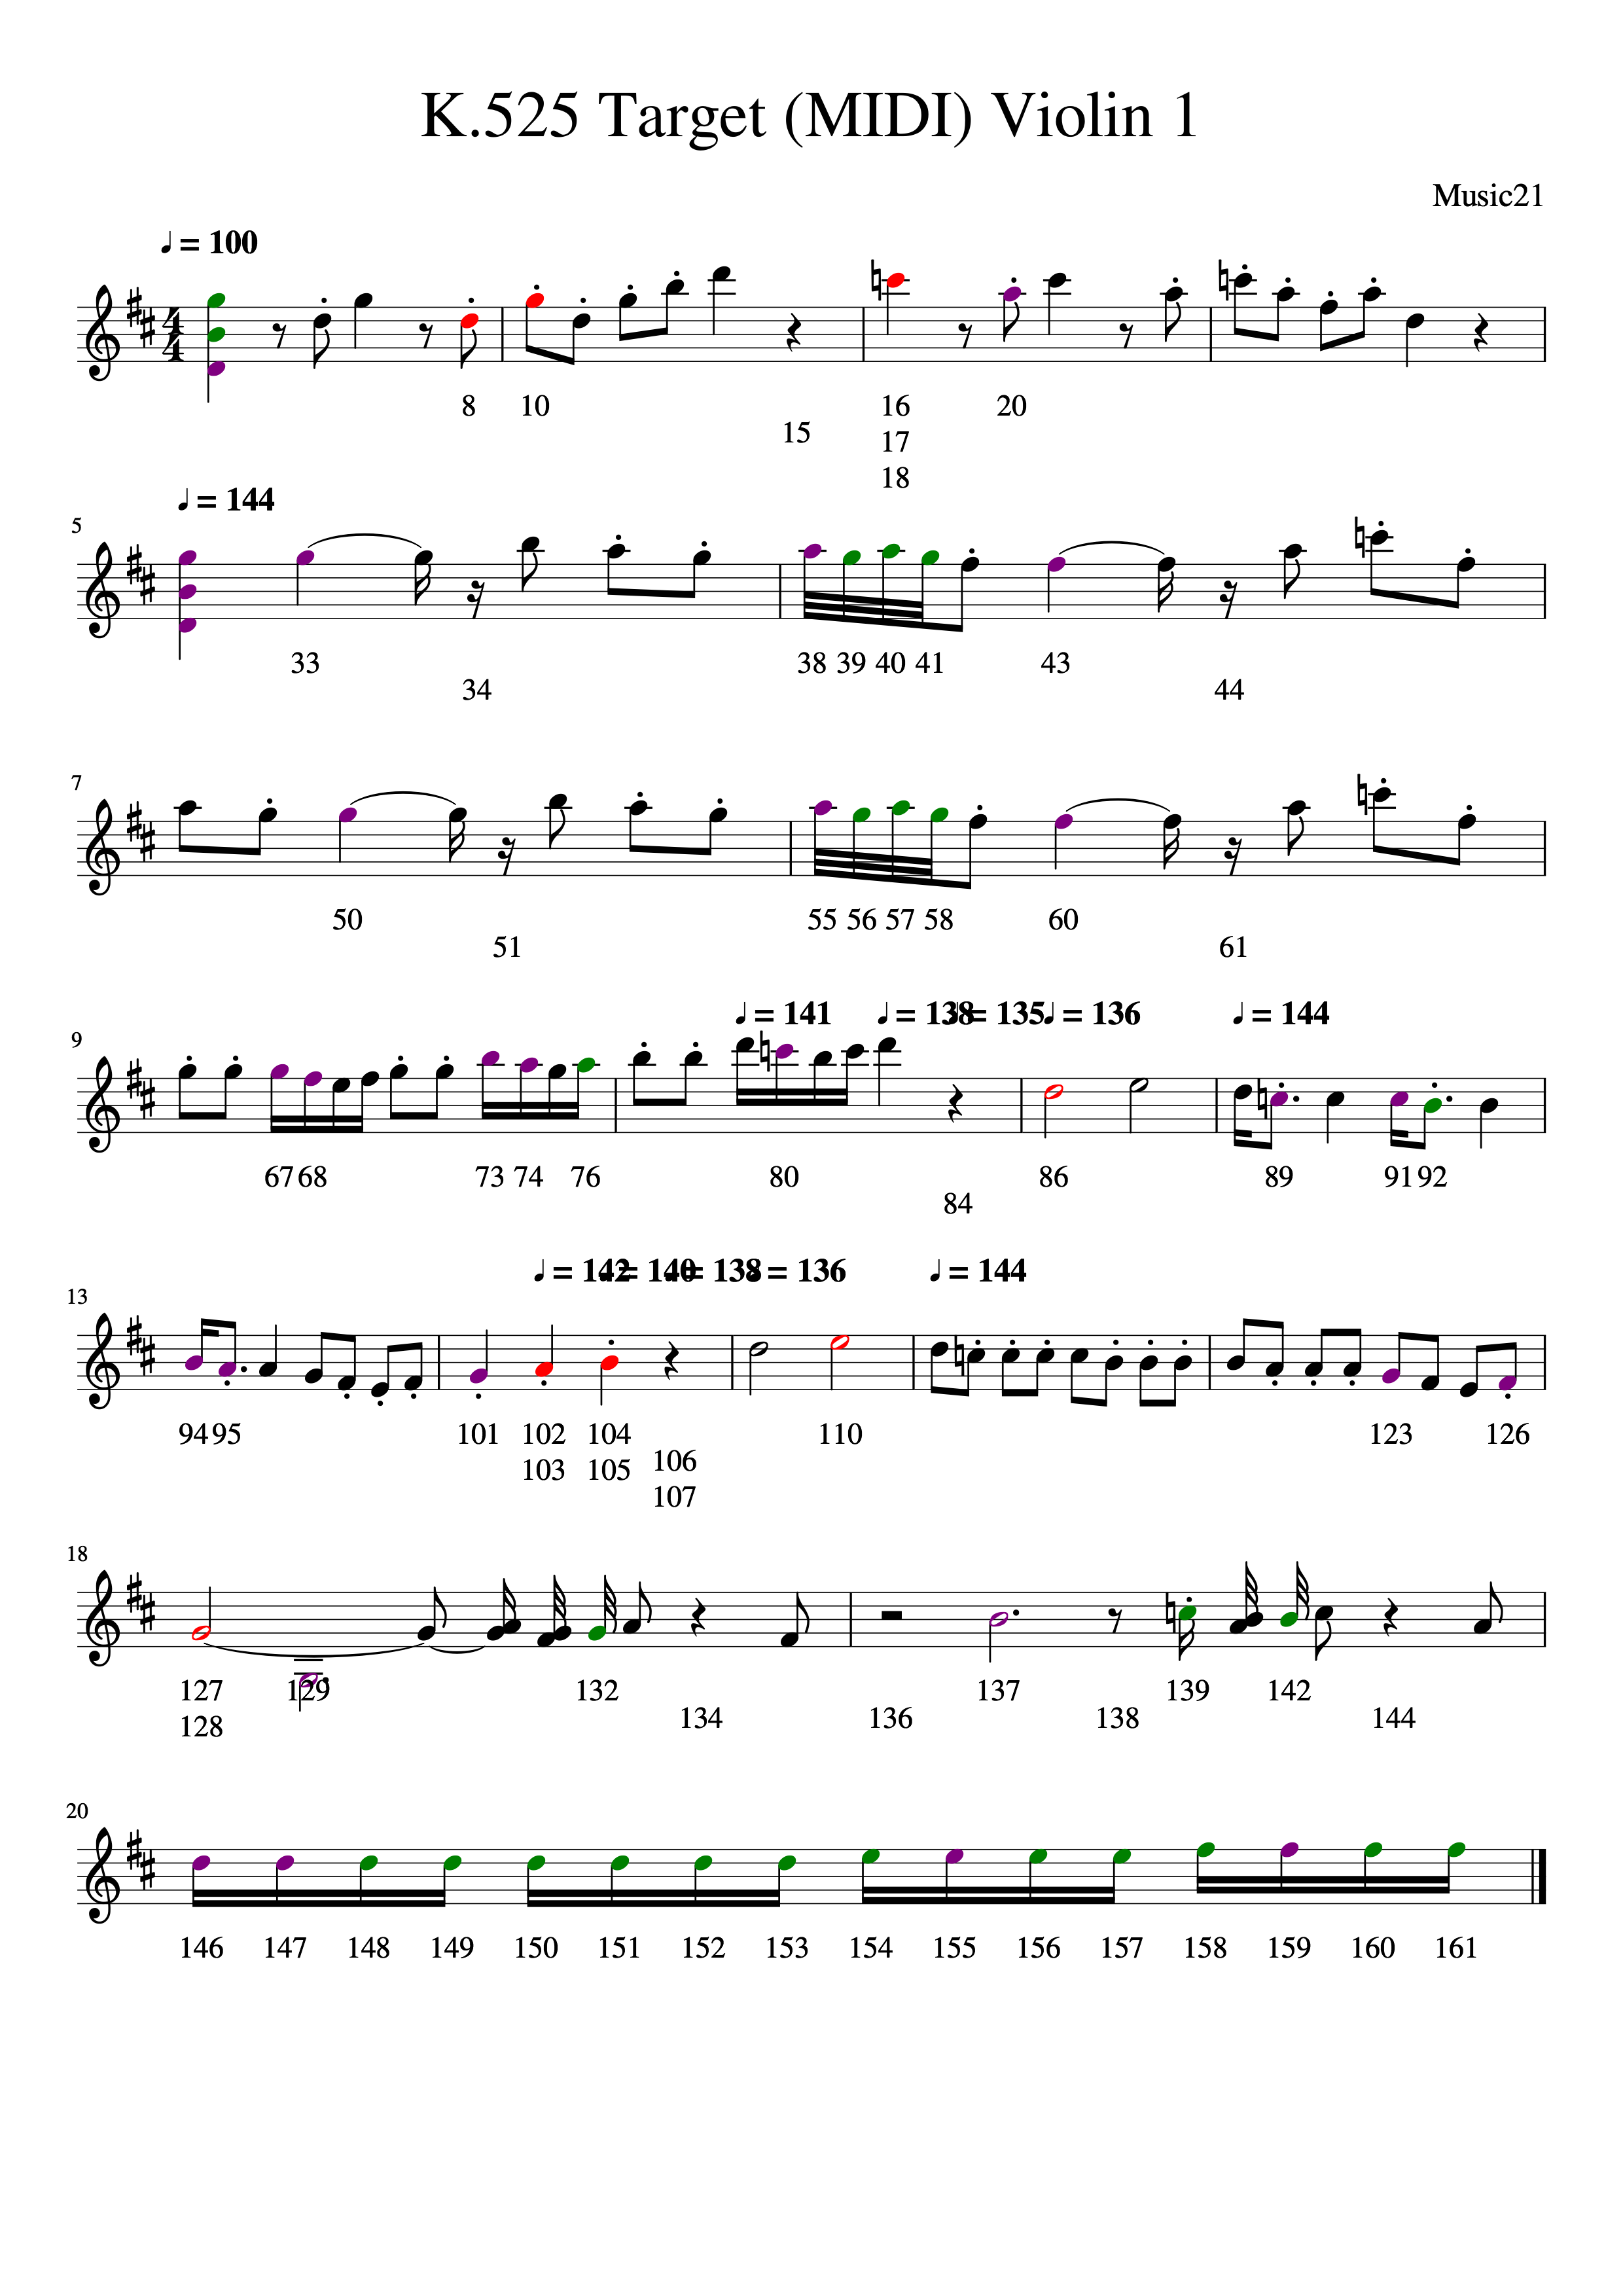
\includegraphics[width =.9\textwidth]{k525postalignV1midi-1}
\caption{Post-alignment visualization of the MIDI Violin 1 part in K.525.}
\end{figure}

\begin{figure}[H]
\centering
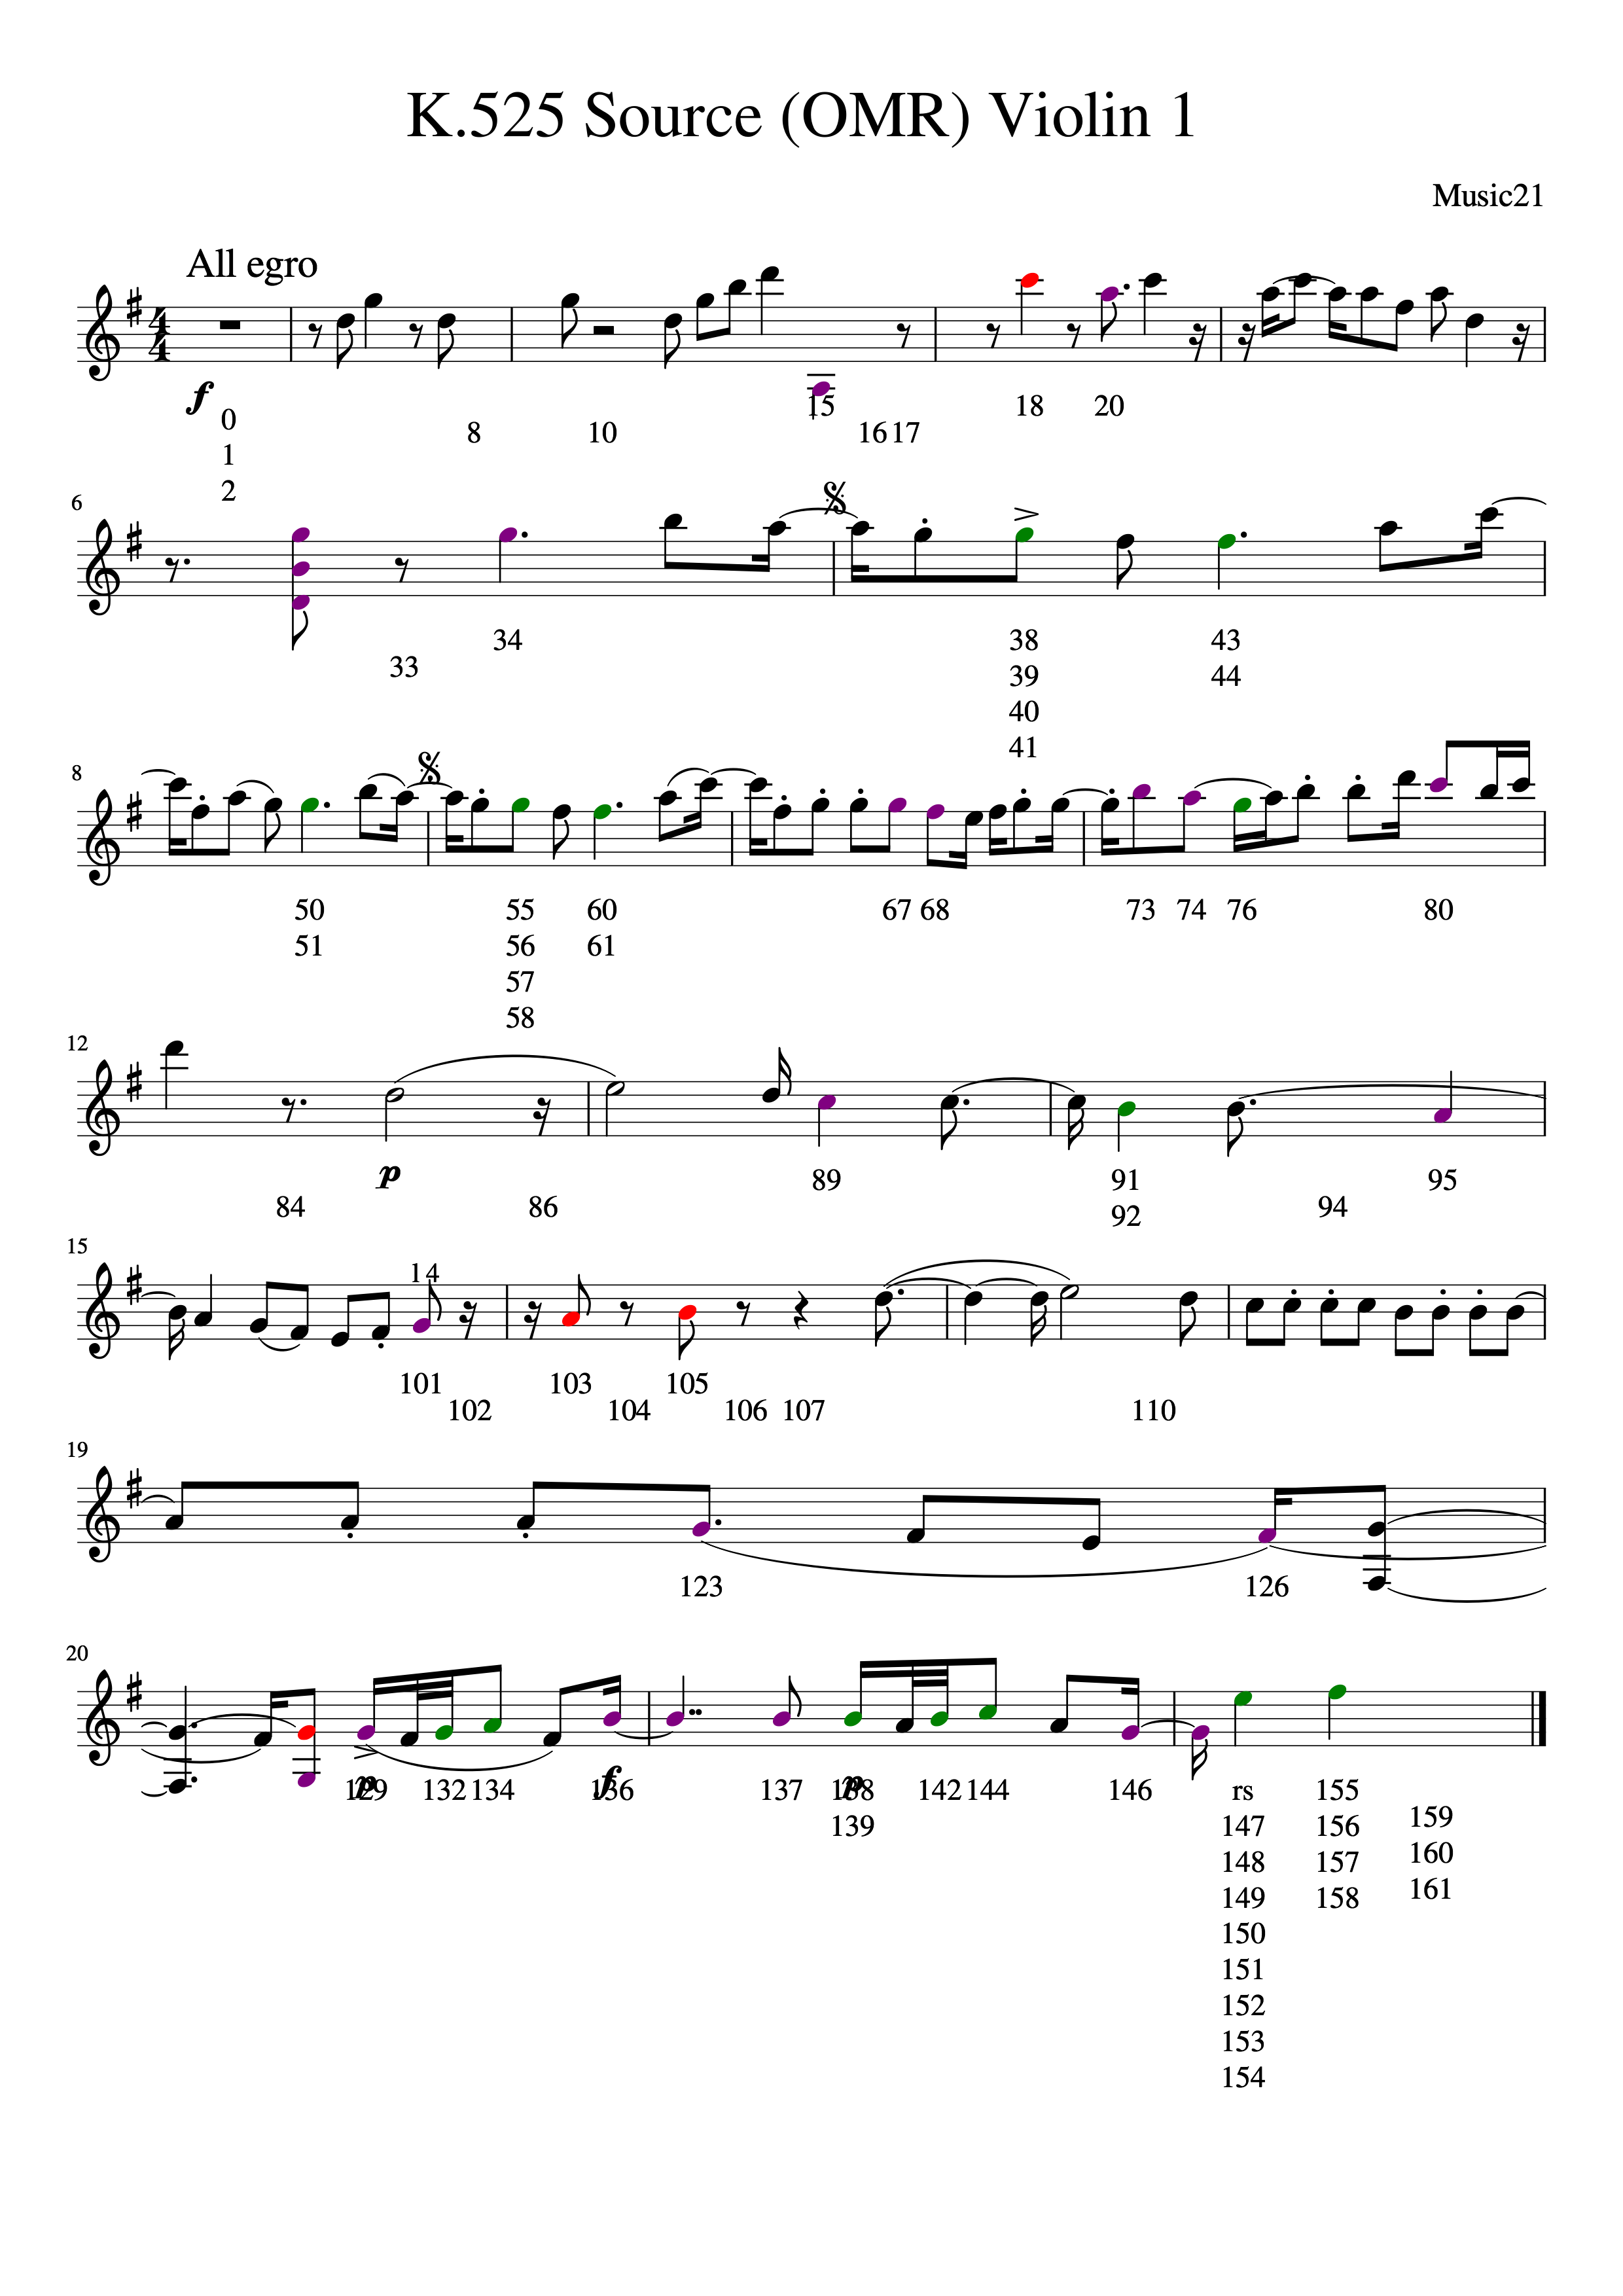
\includegraphics[width =.95\textwidth]{k525postalignV1omr-1}
\caption{Post-alignment visualization of the OMR Violin 1 part in K.525.}
\end{figure}

\begin{figure}[H]
\centering
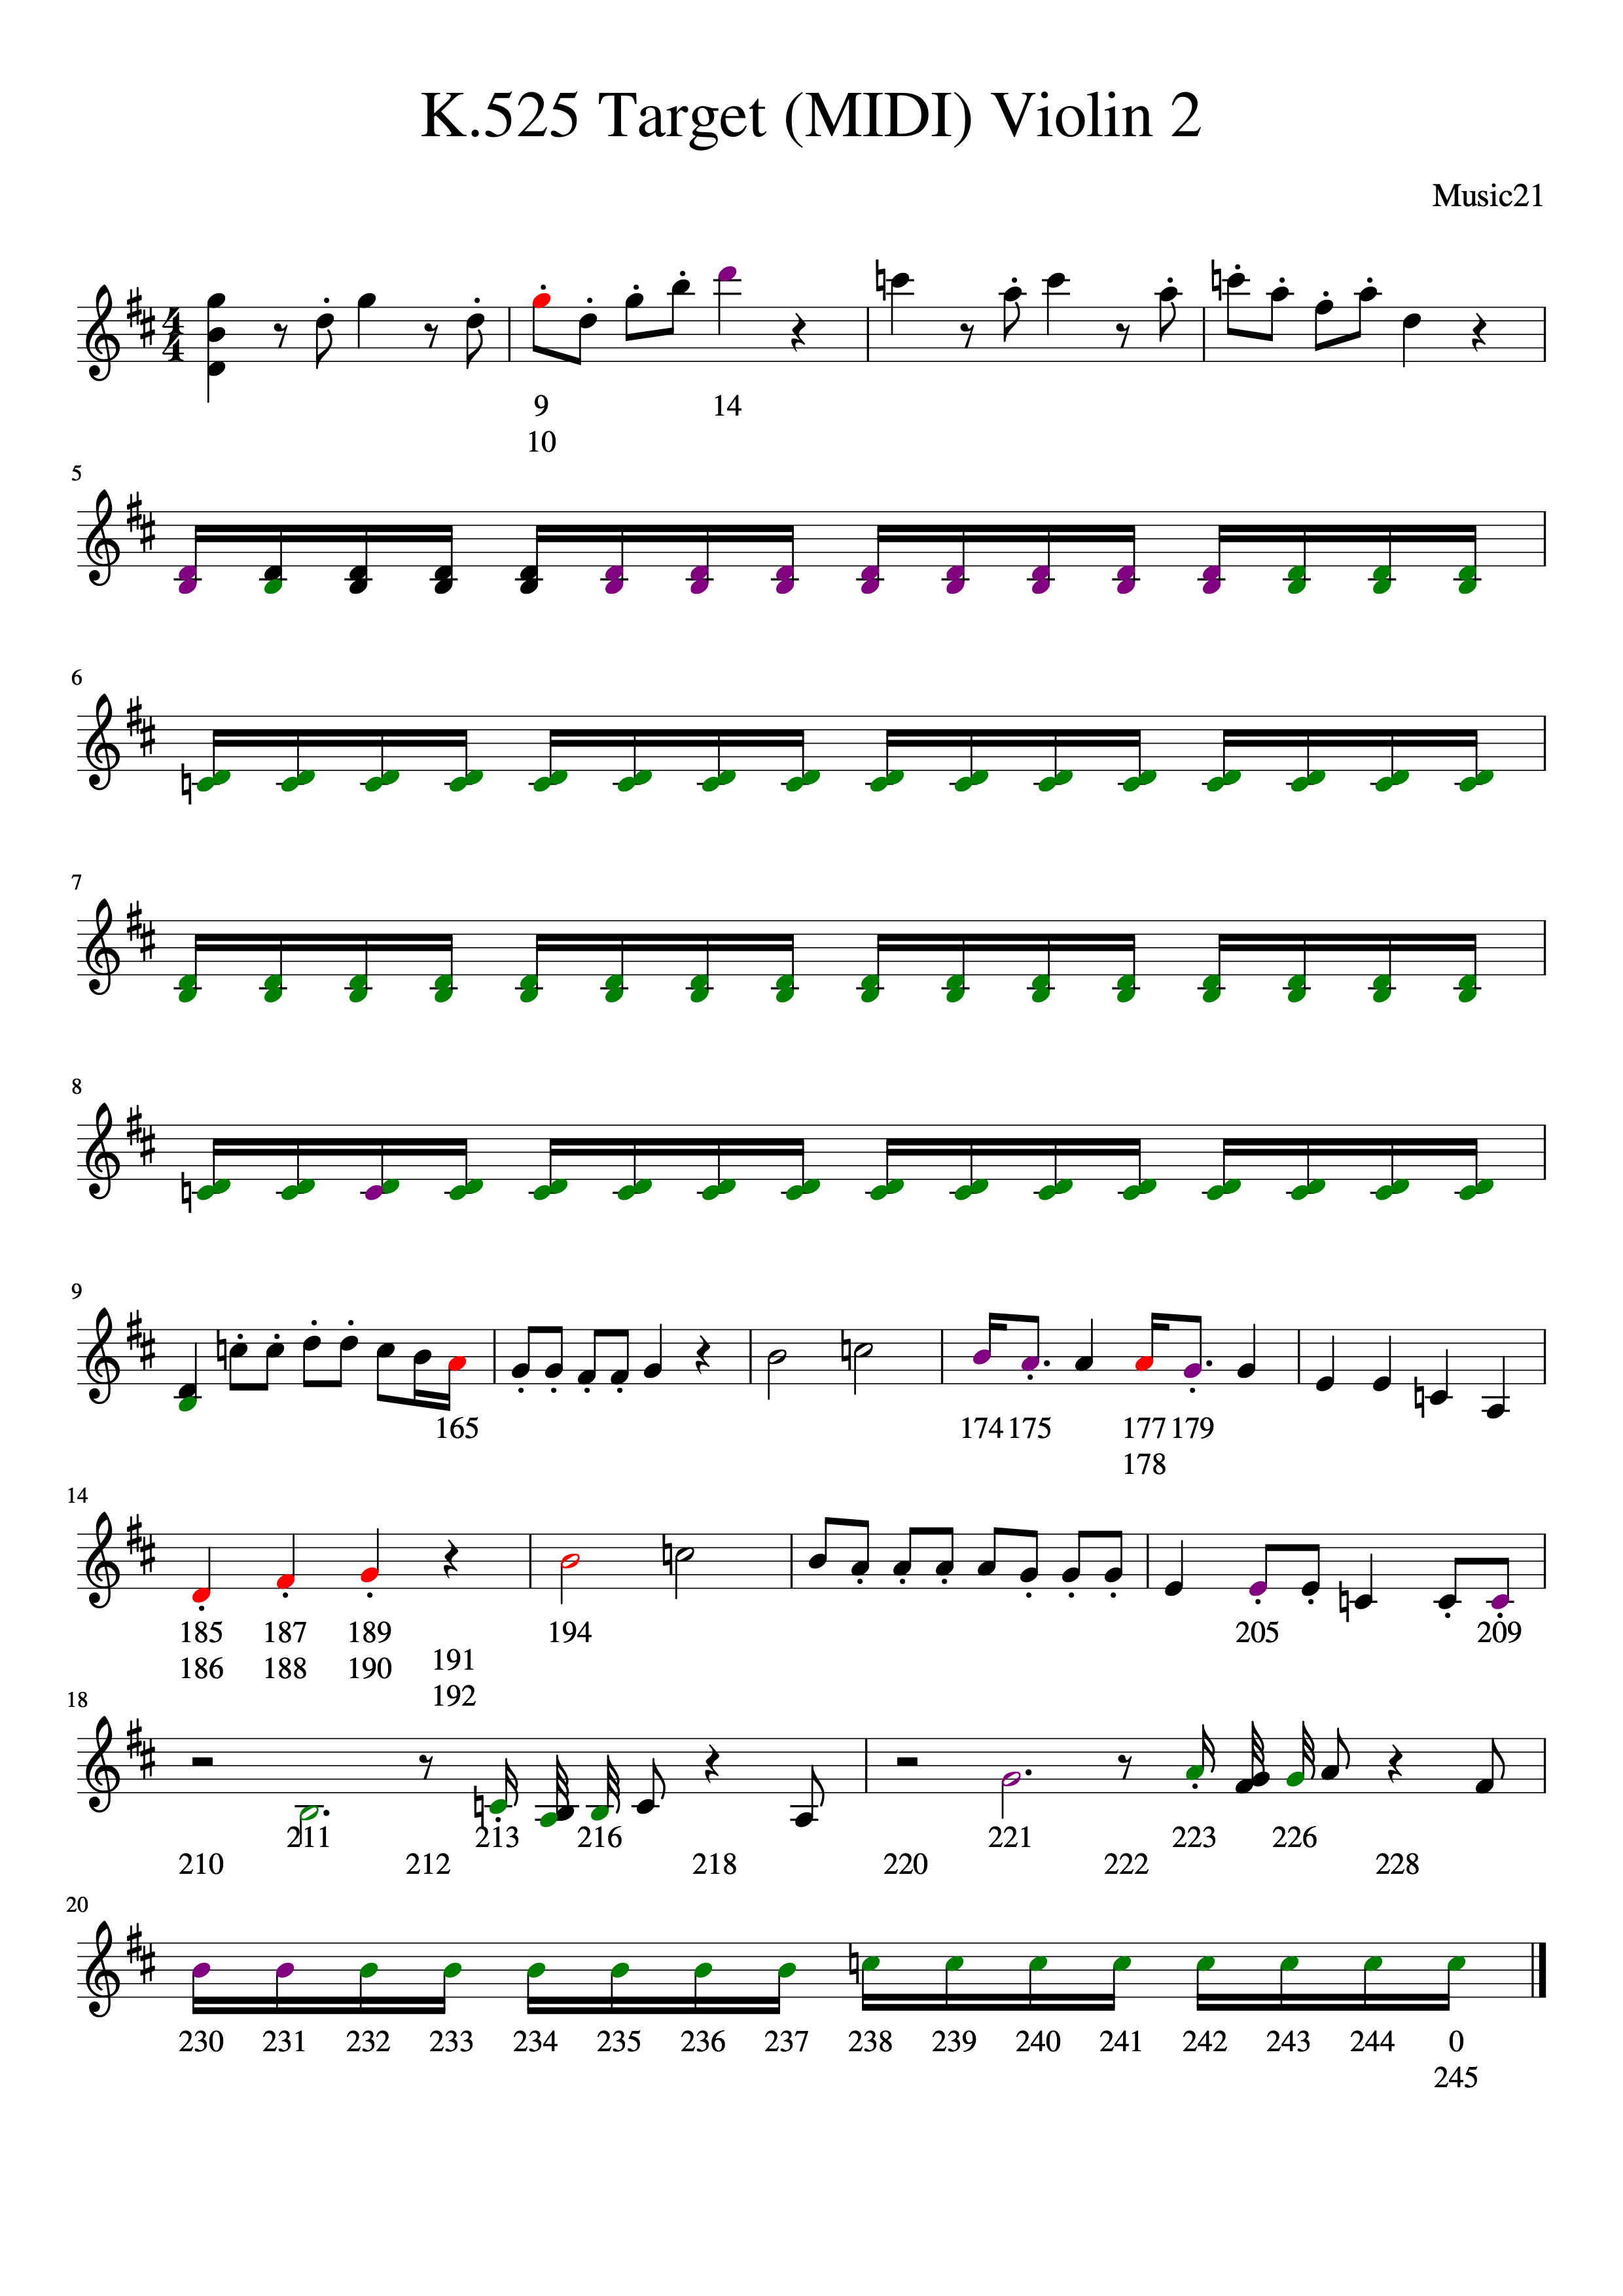
\includegraphics[width =.95\textwidth]{k525postalignV2midi-1}
\caption{Post-alignment visualization of the MIDI Violin 2 part in K.525.}
\end{figure}

\begin{figure}[H]
\centering
\includegraphics[width =.95\textwidth]{k525postalignV2omr-1}
\caption{Post-alignment visualization of the OMR Violin 2 part in K.525.}
\end{figure}

\begin{figure}[H]
\centering
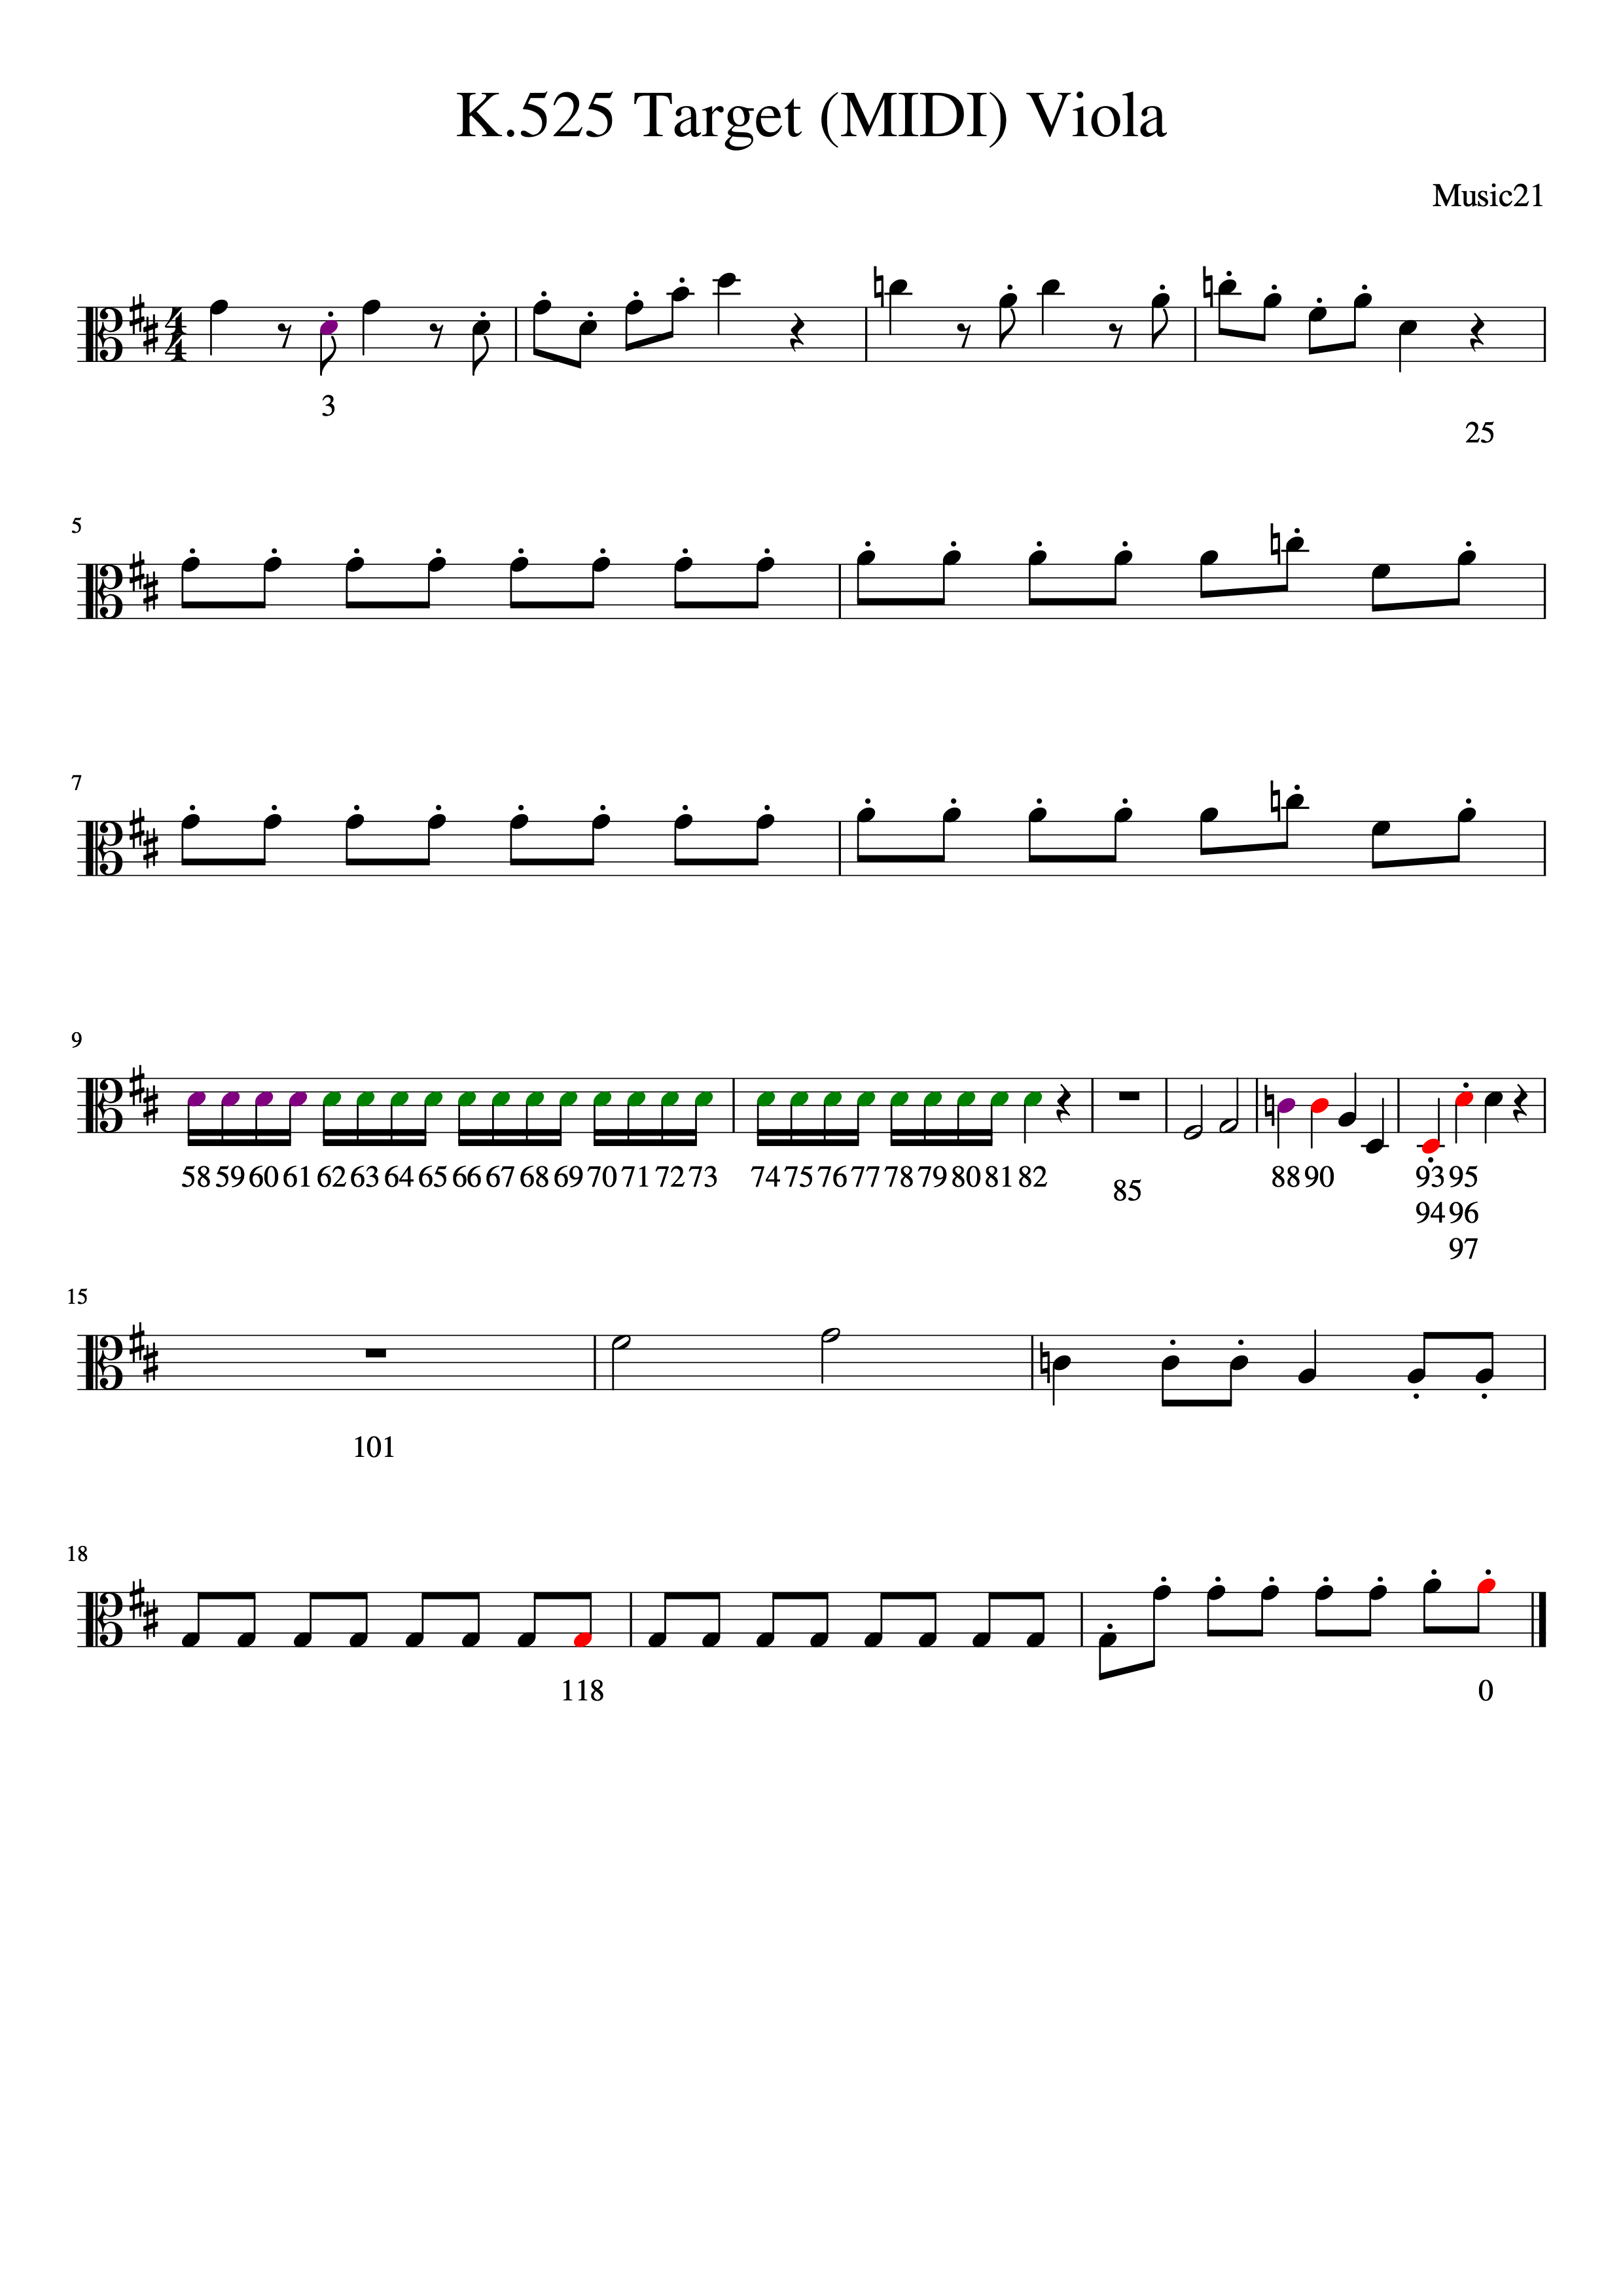
\includegraphics[width =.95\textwidth]{k525postalignviolamidi-1}
\caption{Post-alignment visualization of the MIDI Viola part in K.525.}
\end{figure}

\begin{figure}[H]
\centering
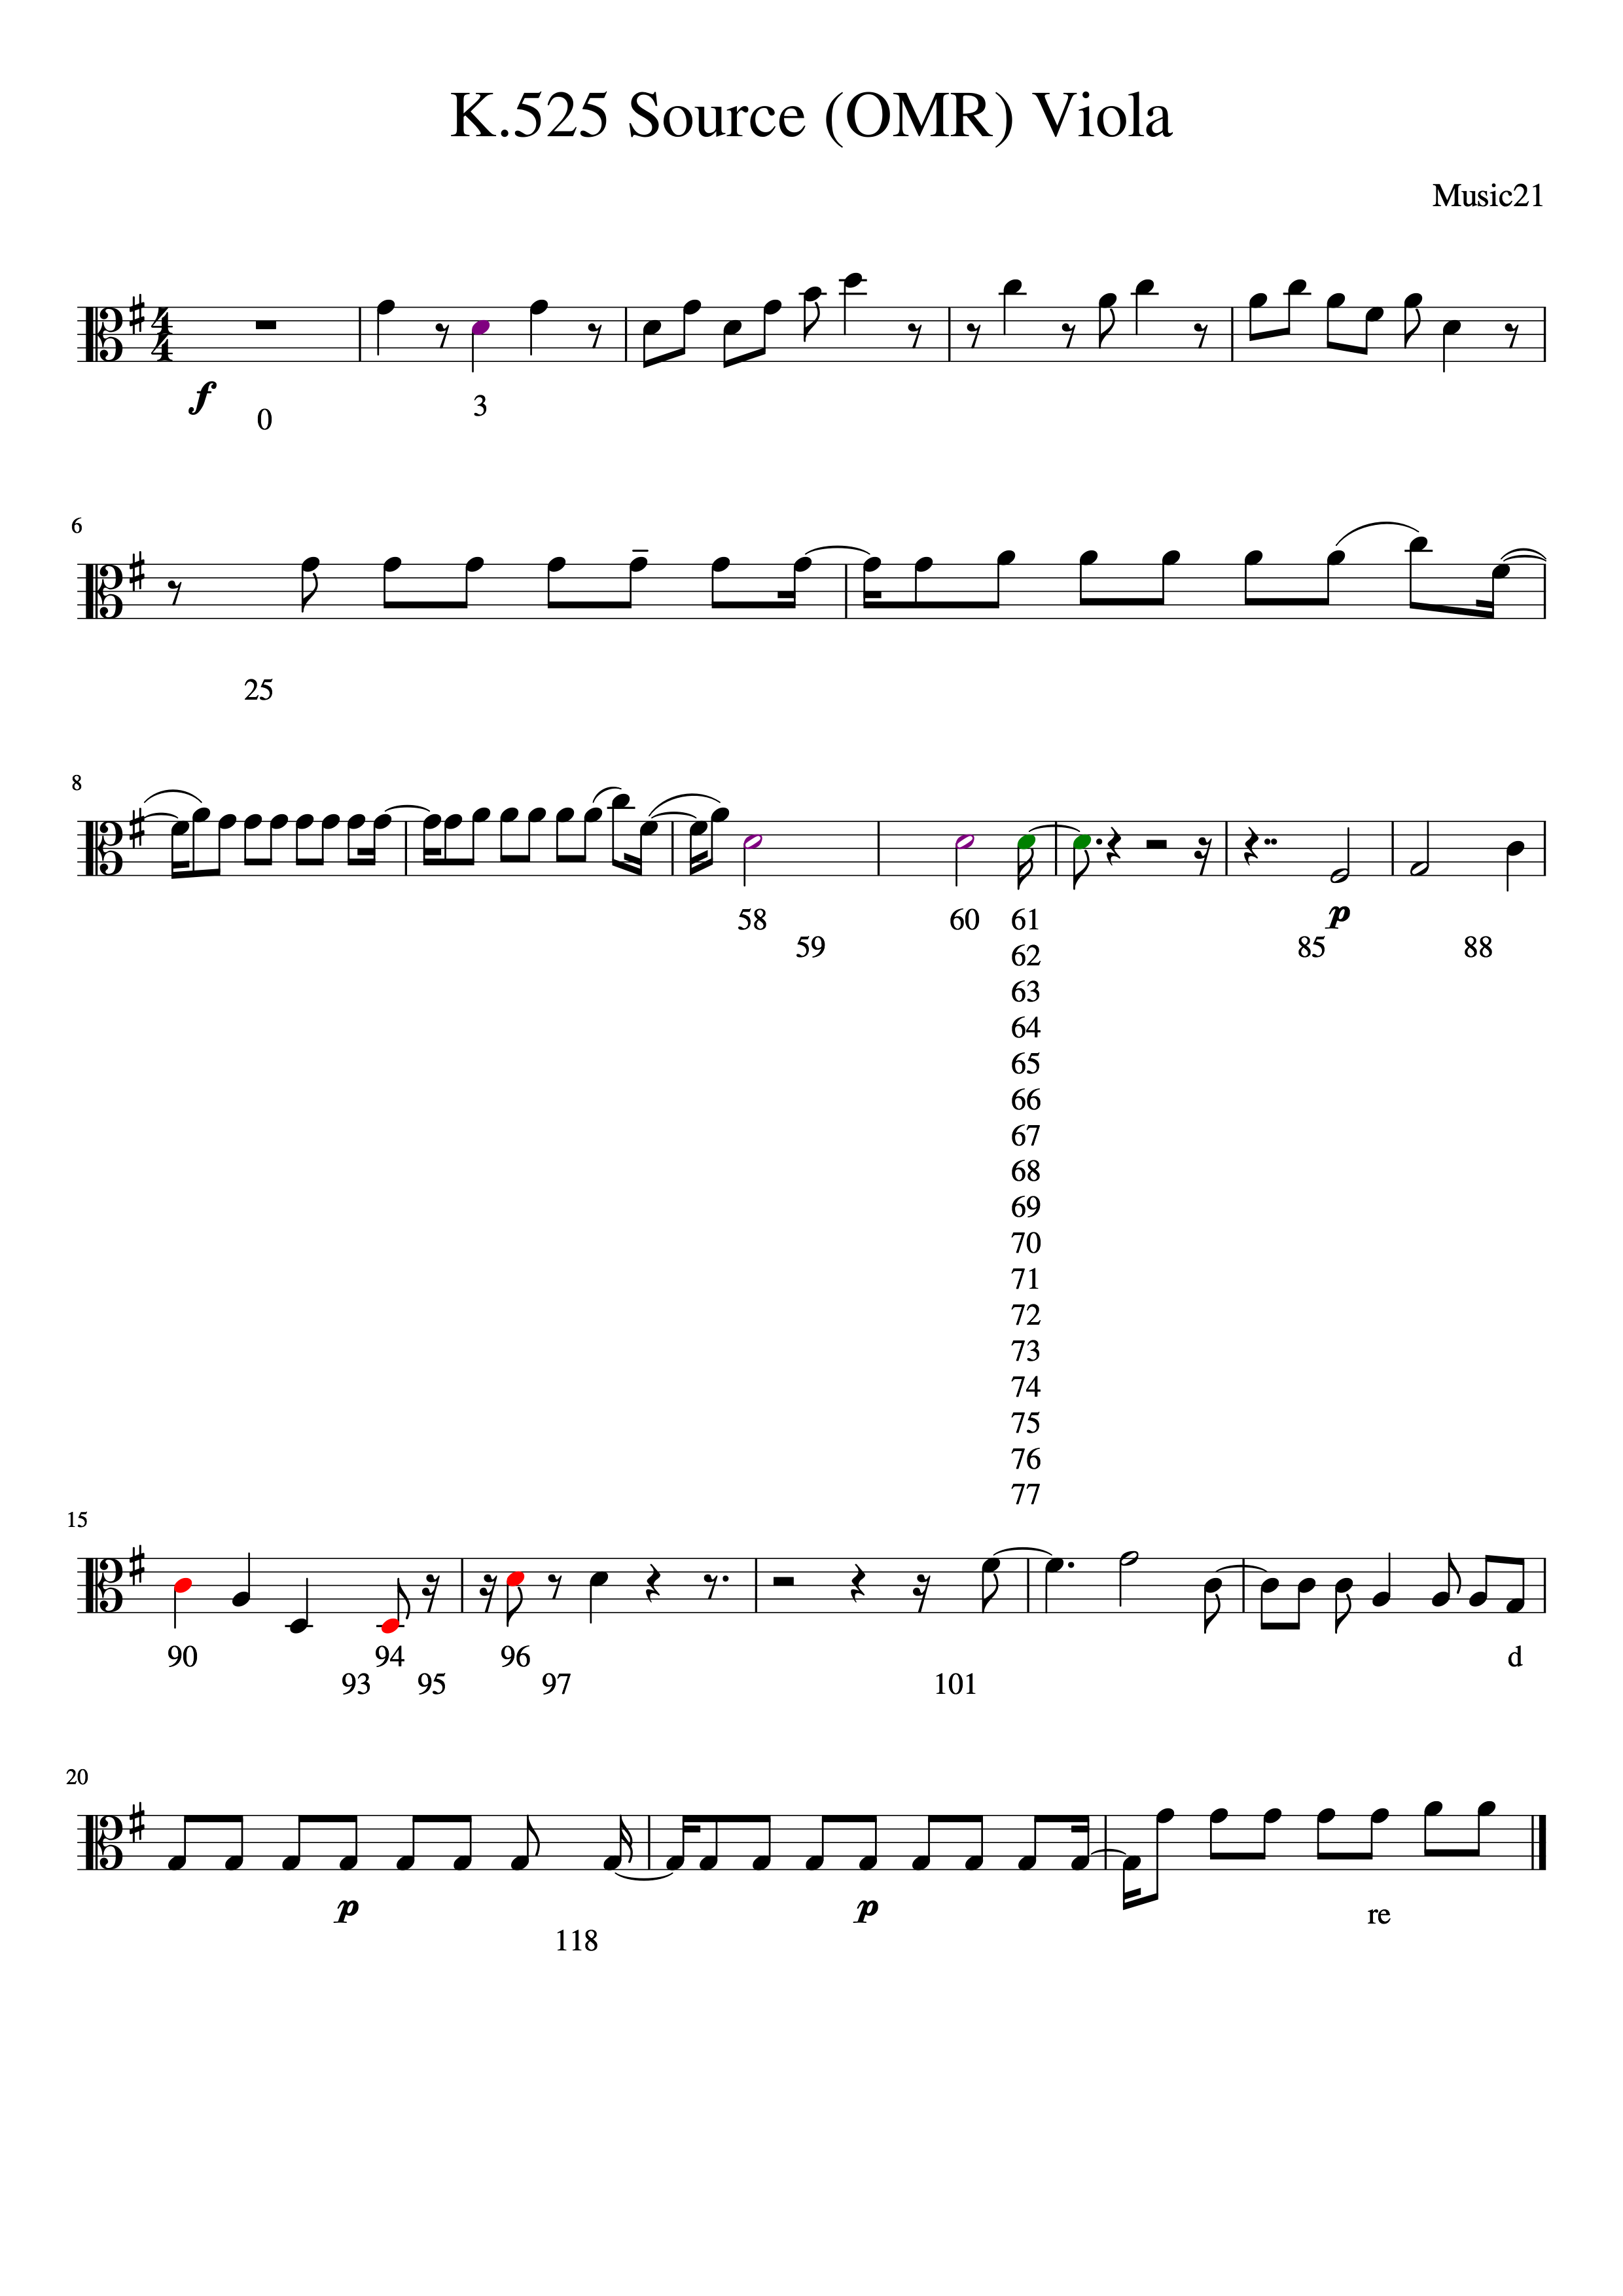
\includegraphics[width =.95\textwidth]{k525postalignviolaomr-1}
\caption{Post-alignment visualization of the OMR Viola part in K.525.}
\end{figure}

\begin{figure}[H]
\centering
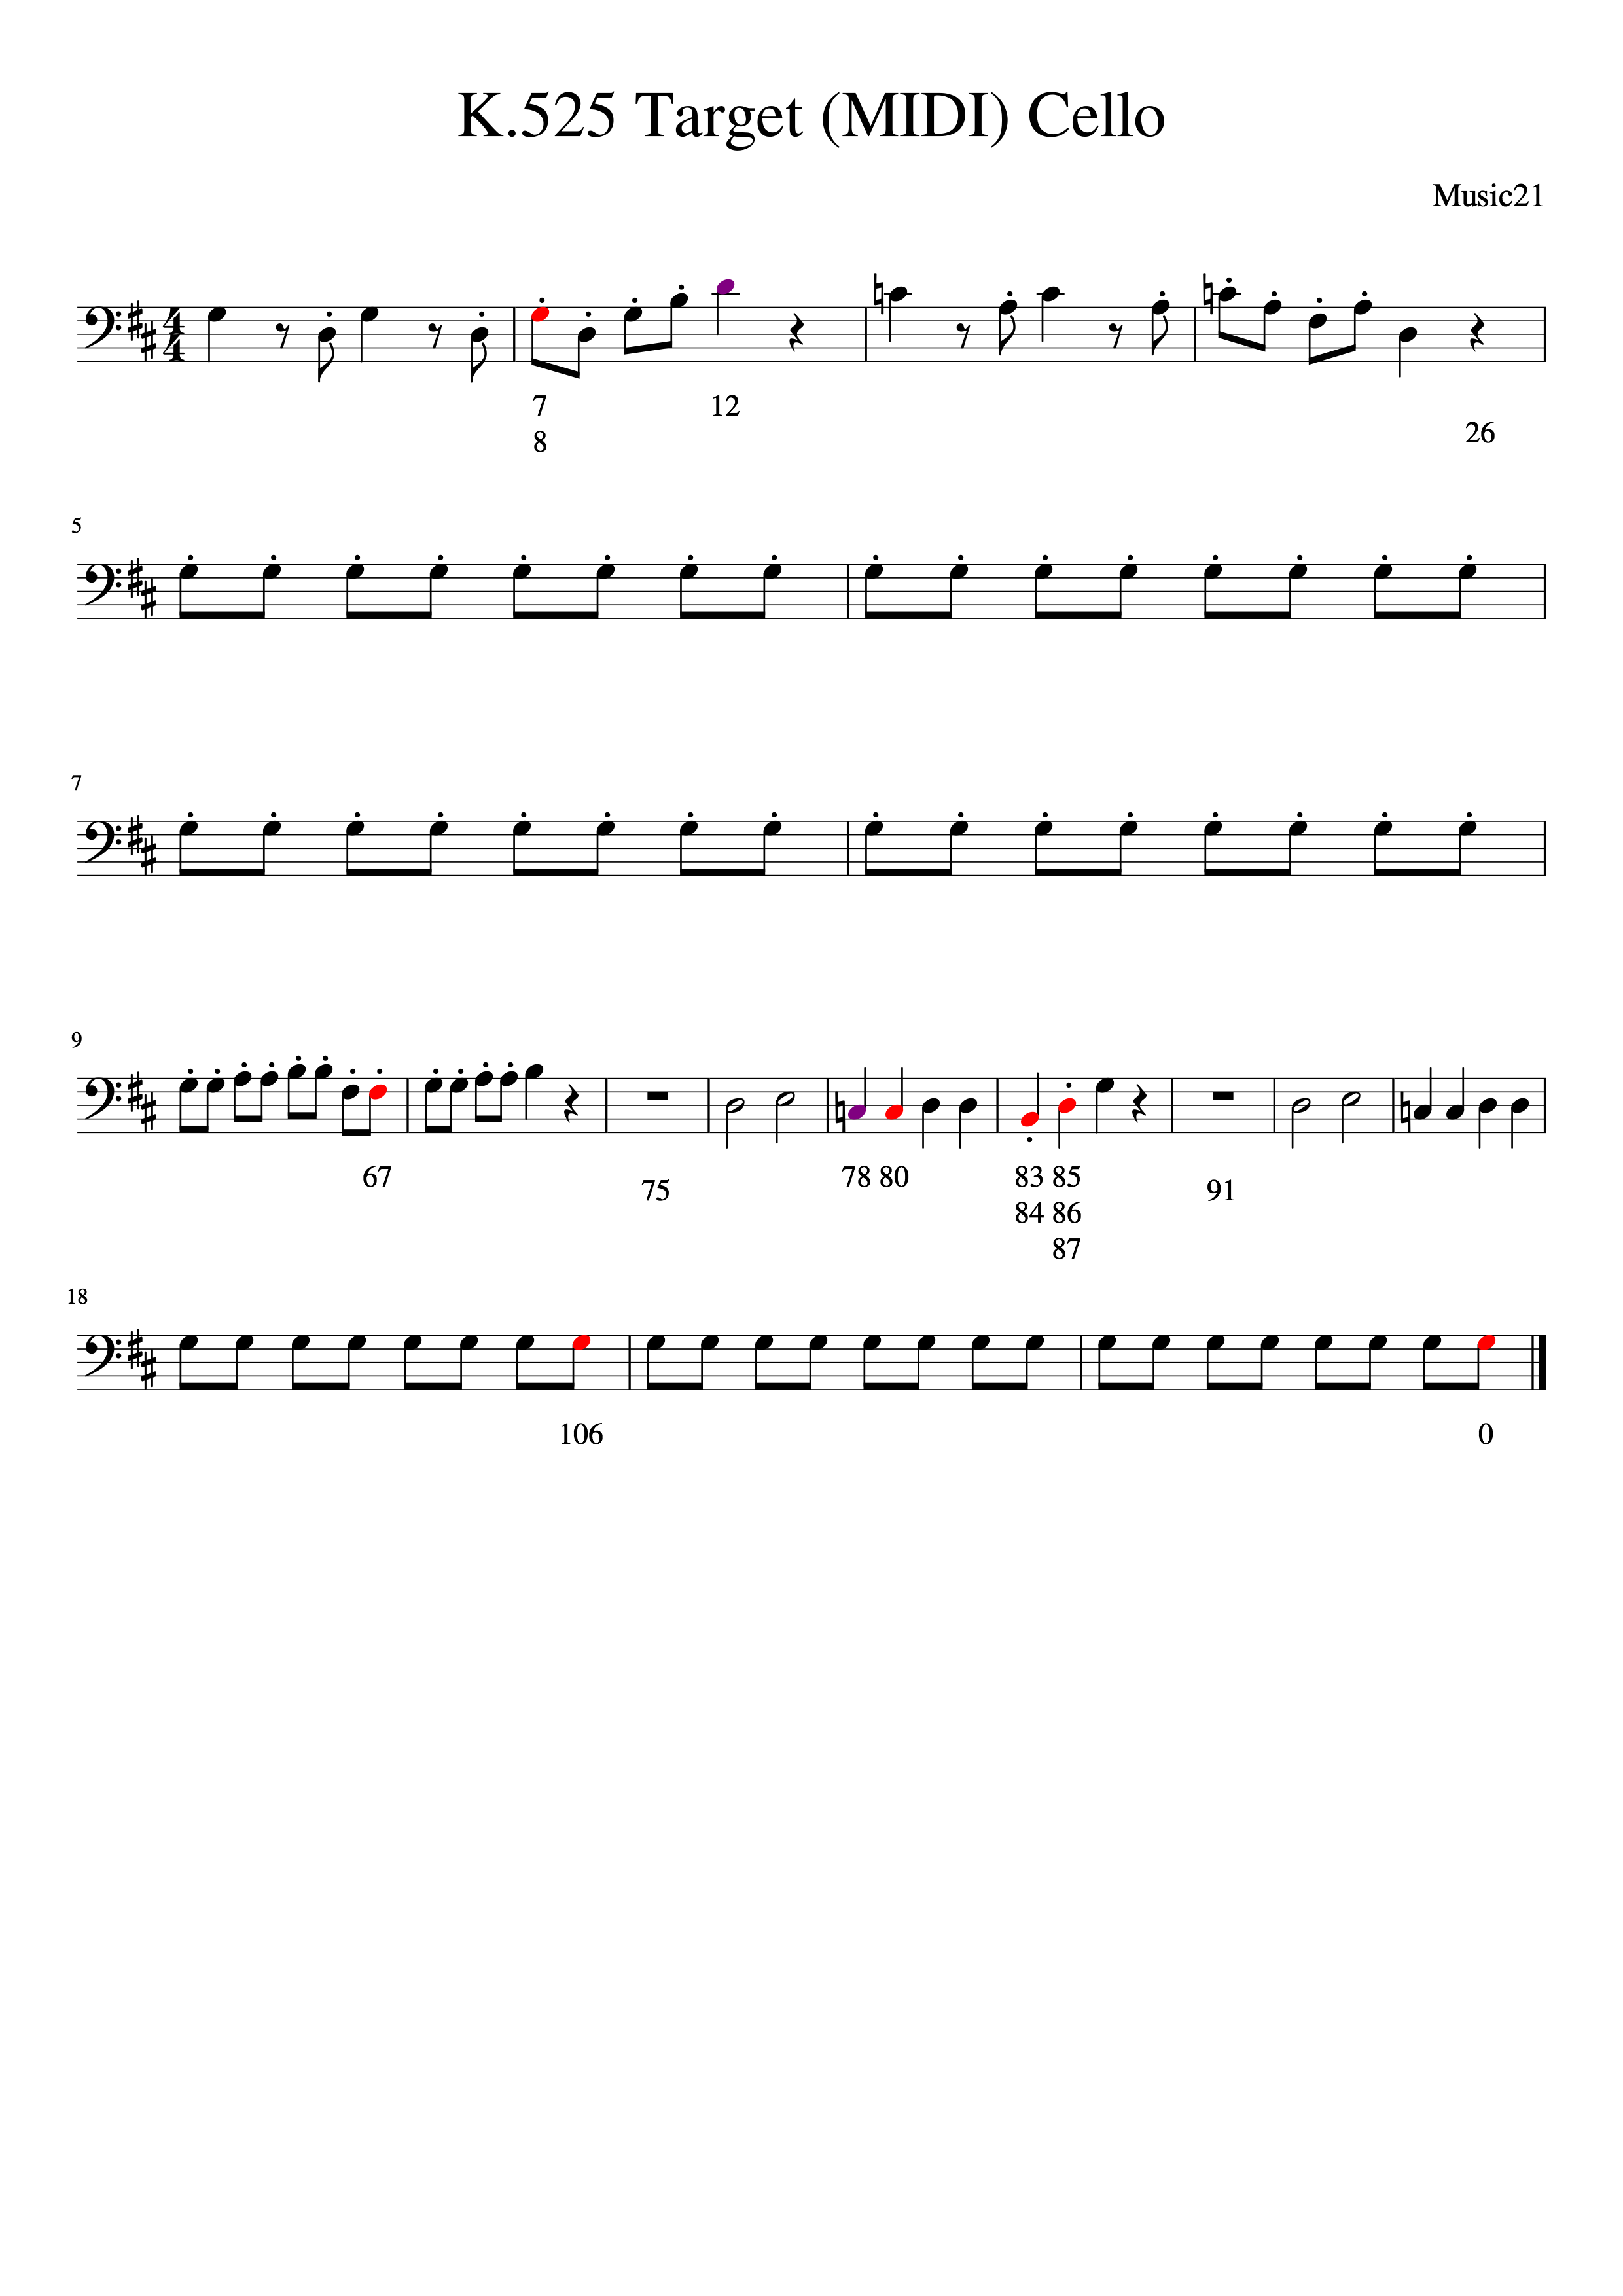
\includegraphics[width =.95\textwidth]{k525postaligncellomidi-1}
\caption{Post-alignment visualization of the MIDI Cello part in K.525.}
\end{figure}

\begin{figure}[H]
\centering
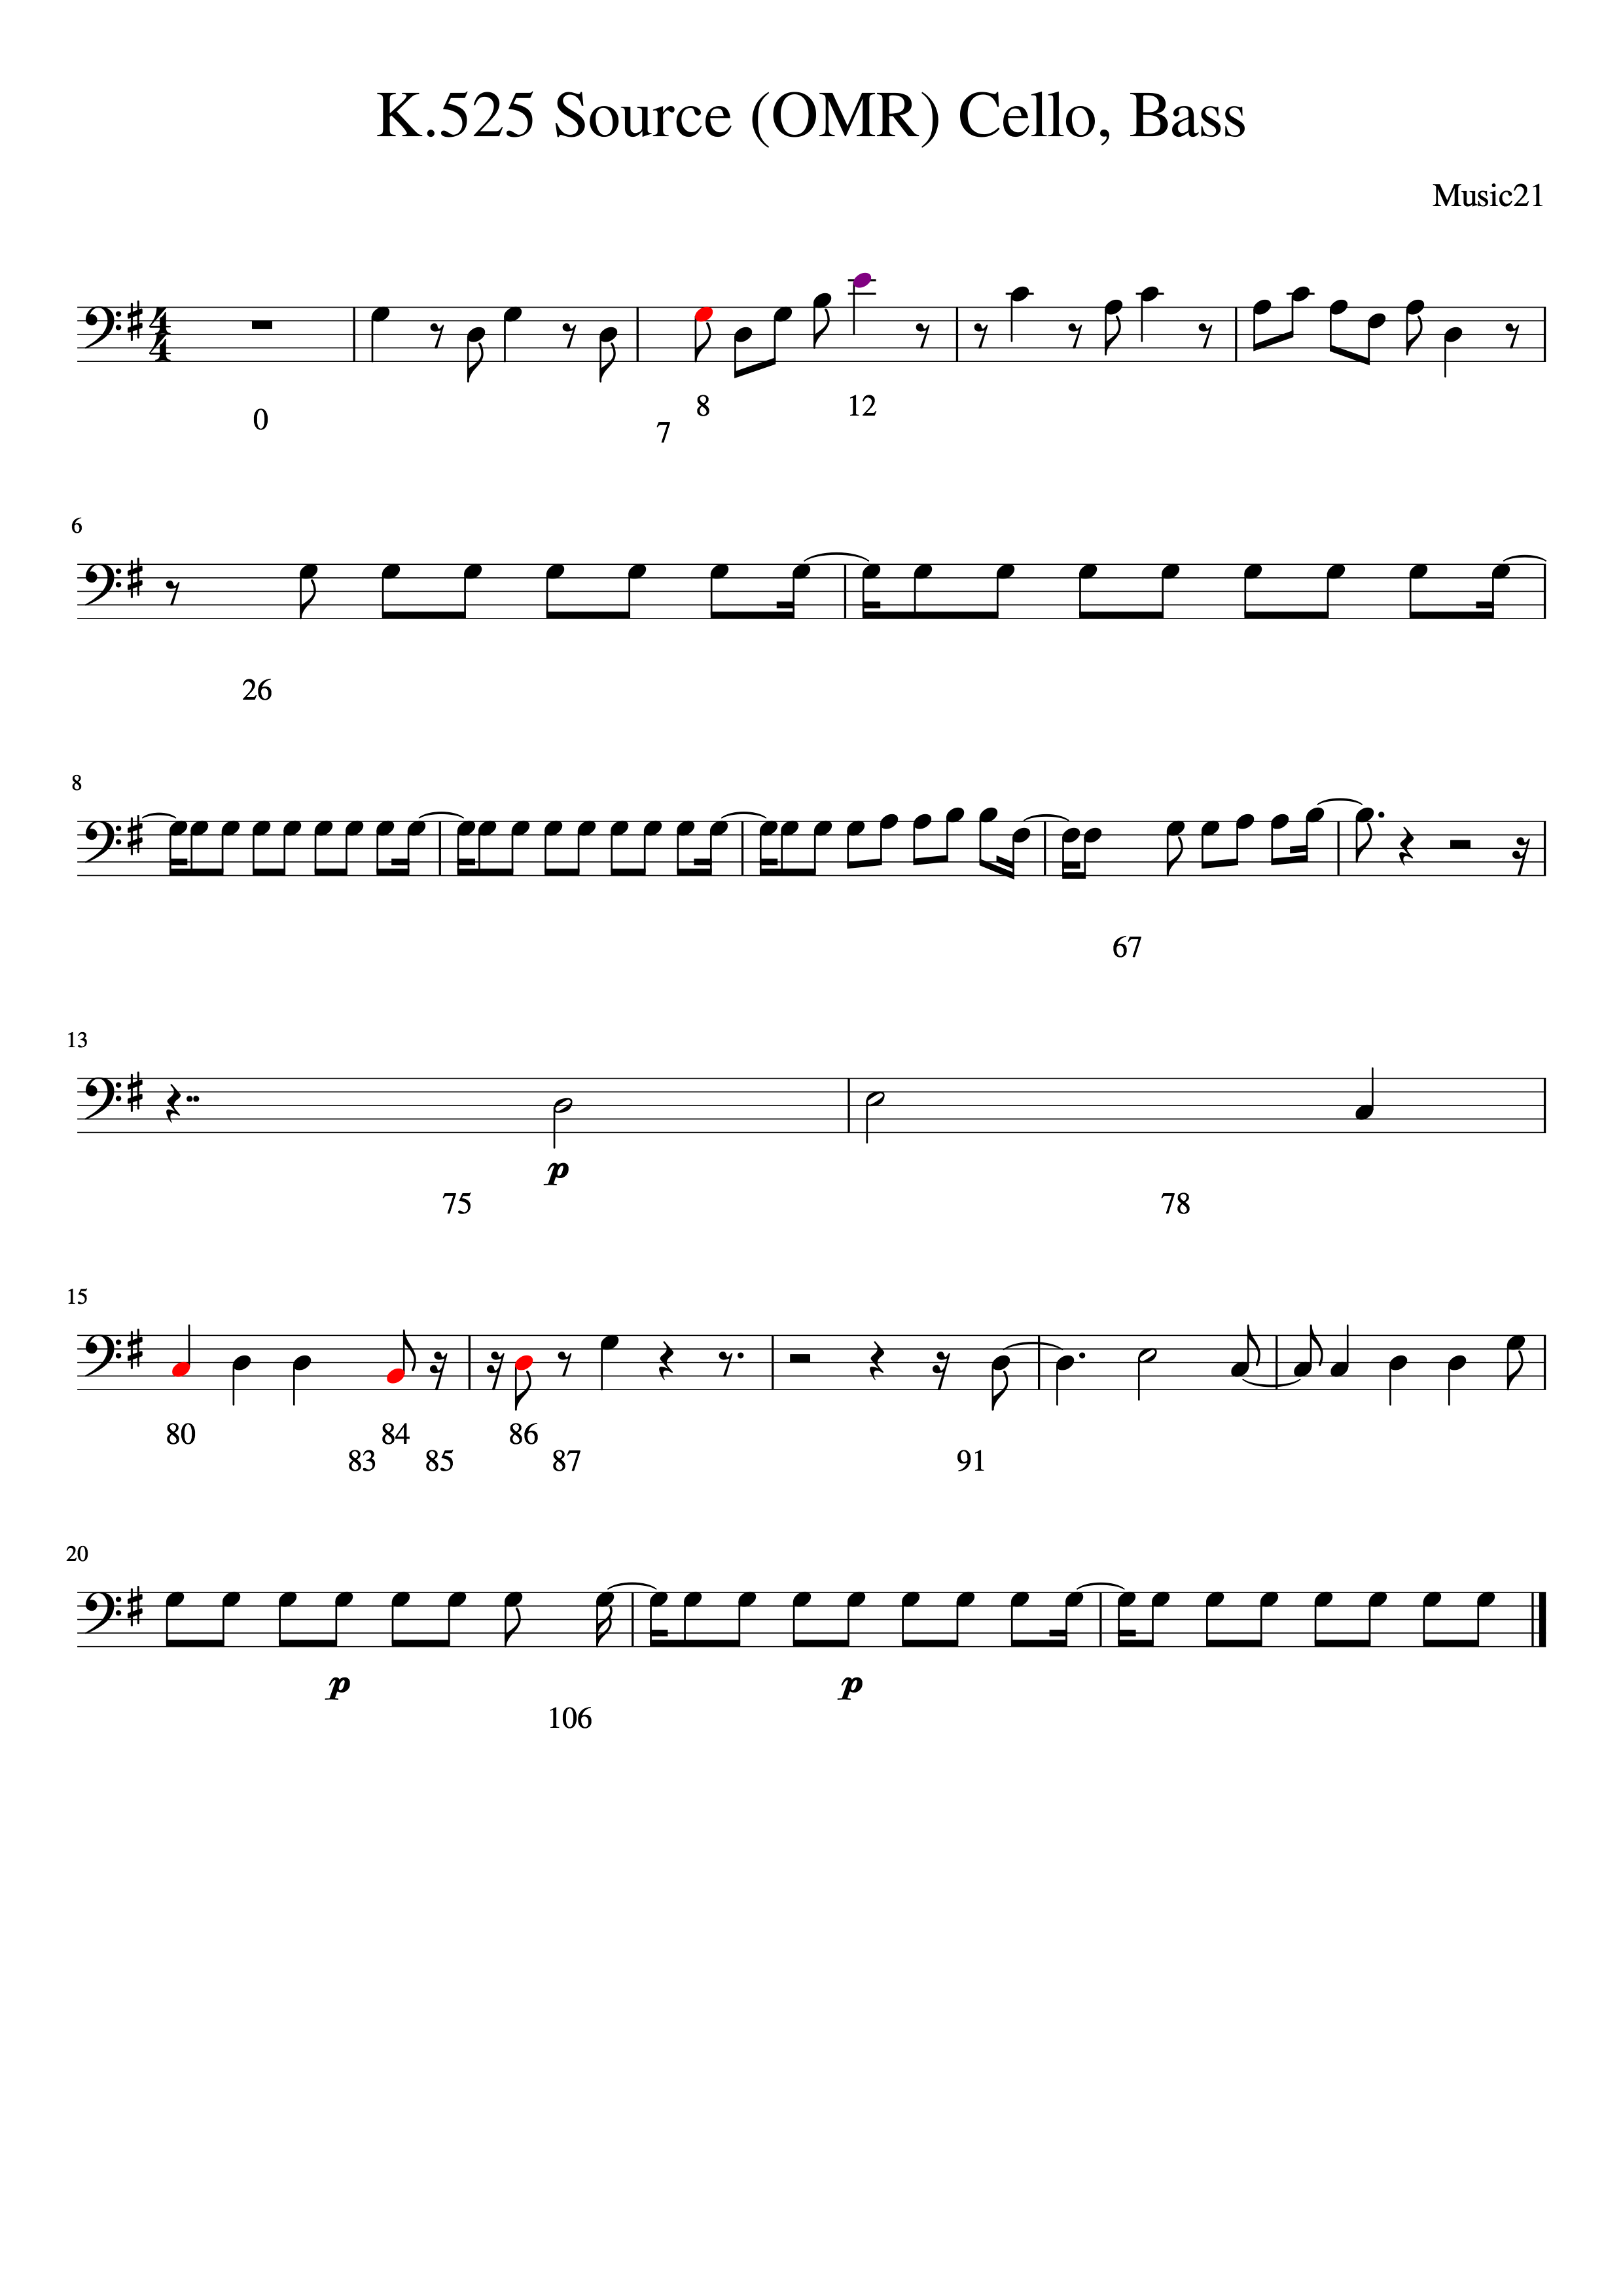
\includegraphics[width =.95\textwidth]{k525postaligncellobassomr-1}
\caption{Post-alignment visualization of the OMR Cello and Bass part in K.525.}
\end{figure}

\subsubsection{A Closer Look at Specifics of \texttt{processrunner}}
A lot of magic happens within \texttt{processRunner}, all of which is described at a high level in sections \ref{processrunner1} - \ref{processrunner2}. Here are some salient details of the process in the context of K.525 that I think deserve notice:
\begin{itemize}
\item Bass Doubles Cello Part - The OMR score has only four parts, whereas the MIDI score has 5. The \texttt{checkBassDoublesCello} method in \texttt{OMRMIDICorrector} is able to correctly identify this and thus does not reject the input on the basis of having a mismatching number of parts in the stream. 
\item Rhythmic Fault Tolerance: Beginning Rests - The first measure in the OMR score is a scanning and parsing error. The \texttt{Aligner} is robust enough to identify the beginning rest as a insertion error. 
\item Rhythmic Fault Tolerance: Propagating Rhythmic Shifts - By measure 5, we see that the OMR score has introduced a \nth{16} note shift in the rhythm which continues for a few measures. 
\item Notation Fault Tolerance: Tremolos - By measure 5 of the violin 2 part and by measure 10 of the Viola part, the repeated \nth{16} notes get notated with tremolo slashes in the original OMR score. Of course, the MIDI protocol doesn't have a way of representing tremolo, so the notes are written out in long form. The corrector is able to match the written out repeated notes in the MIDI to the (incorrectly) scanned corresponding notes in the OMR. 
\end{itemize}

\subsection{Similarity Metrics}
Recall that the \texttt{similarityScore} is the ratio of \texttt{NoChange} operations to the total number of operations in the \texttt{changes} list. For each pair of streams in K.525, the \texttt{similarityScore} and \texttt{changesCount} are listed below:
\begin{table}[H]
\centering
\begin{tabular}{lll}
           & \texttt{similarityScore} & \texttt{changesCount}                                                  \\
Violin 1   & 0.51                       & \{NoChange: 83, Ins: 30, Del: 10, Sub: 39\} \\
Violin 2   & 0.30                       & \{NoChange: 74, Ins: 125, Del: 9, Sub: 38\} \\
Viola      & 0.72                       & \{NoChange: 97, Ins: 21, Del: 9, Sub: 8\}   \\
Cello/Bass & 0.87                       & \{NoChange: 107, Del: 11, Sub: 5\}               
\end{tabular}
\caption{\texttt{similarityScore} and \texttt{changesCount} for every pair of aligned streams}
\end{table}

A visual examination of the pairs of streams suggests that these numbers and counts look correct. The Cello/Bass parts have the fewest colorations to their notes and no insertion changes at all. The least similar pair of parts is the Violin 2, which has multiple cases of the tremolo problem described above as well as propagating rhythmic shifts.

\section{Example 2: String Quartet No.7 in E-flat major, K.160/159a, K.160, W. A. Mozart)}
This section will go through an example of how just the \texttt{EnharmonicFixer} works on correcting and excerpt of the Violin 1 part of W. A. Mozart's \textit{String Quartet No.7 in E-flat major, K.160, Mvt. I}. The OMR score was sources from IMSLP \cite{k160}.

\subsection{Running \texttt{EnharmonicFixer} on K.160, Violin 1}
After prepping the raw input files of K.160 in the same way as detailed above and running that through an \texttt{OMRMIDICorrector} instance, we will create an and \texttt{EnharmonicFixer} instance using just the Violin 1 OMR stream and MIDI stream and the associated \texttt{changes} list.

\begin{minted}{python}
from music21 import *
k160iMidiFilepath = "pathto/k160/miditoxml.xml"
k160iOmrFilepath = "pathto/k160/omrtoxml.xml"
         
k160midiStream = converter.parse(k160iMidiFilepath)
k160omrStream = converter.parse(k160iOmrFilepath)
k160omc = OMRMIDICorrector(k160midiStream, k160omrStream)
k160omc.processRunner()
        
k160omcV1Changes = k160omc.changes[0]
k160omcV1Midi = k160omc.midiParts[0]
k160omcV1Omr = k160omc.omrParts[0]
k160EF = fixer.EnharmonicFixer(k160omcV1Changes, k160omcV1Midi, k160omcV1Omr)
k160EF.fix()

k160omcViolin1OmrStream.show()
\end{minted}

The first two figures below show the alignment visualization of the Violin 1 part. The last figure shows the corrected OMR score after it has been changed by the \texttt{EnharmonicFixer}

\begin{figure}[H]
\centering
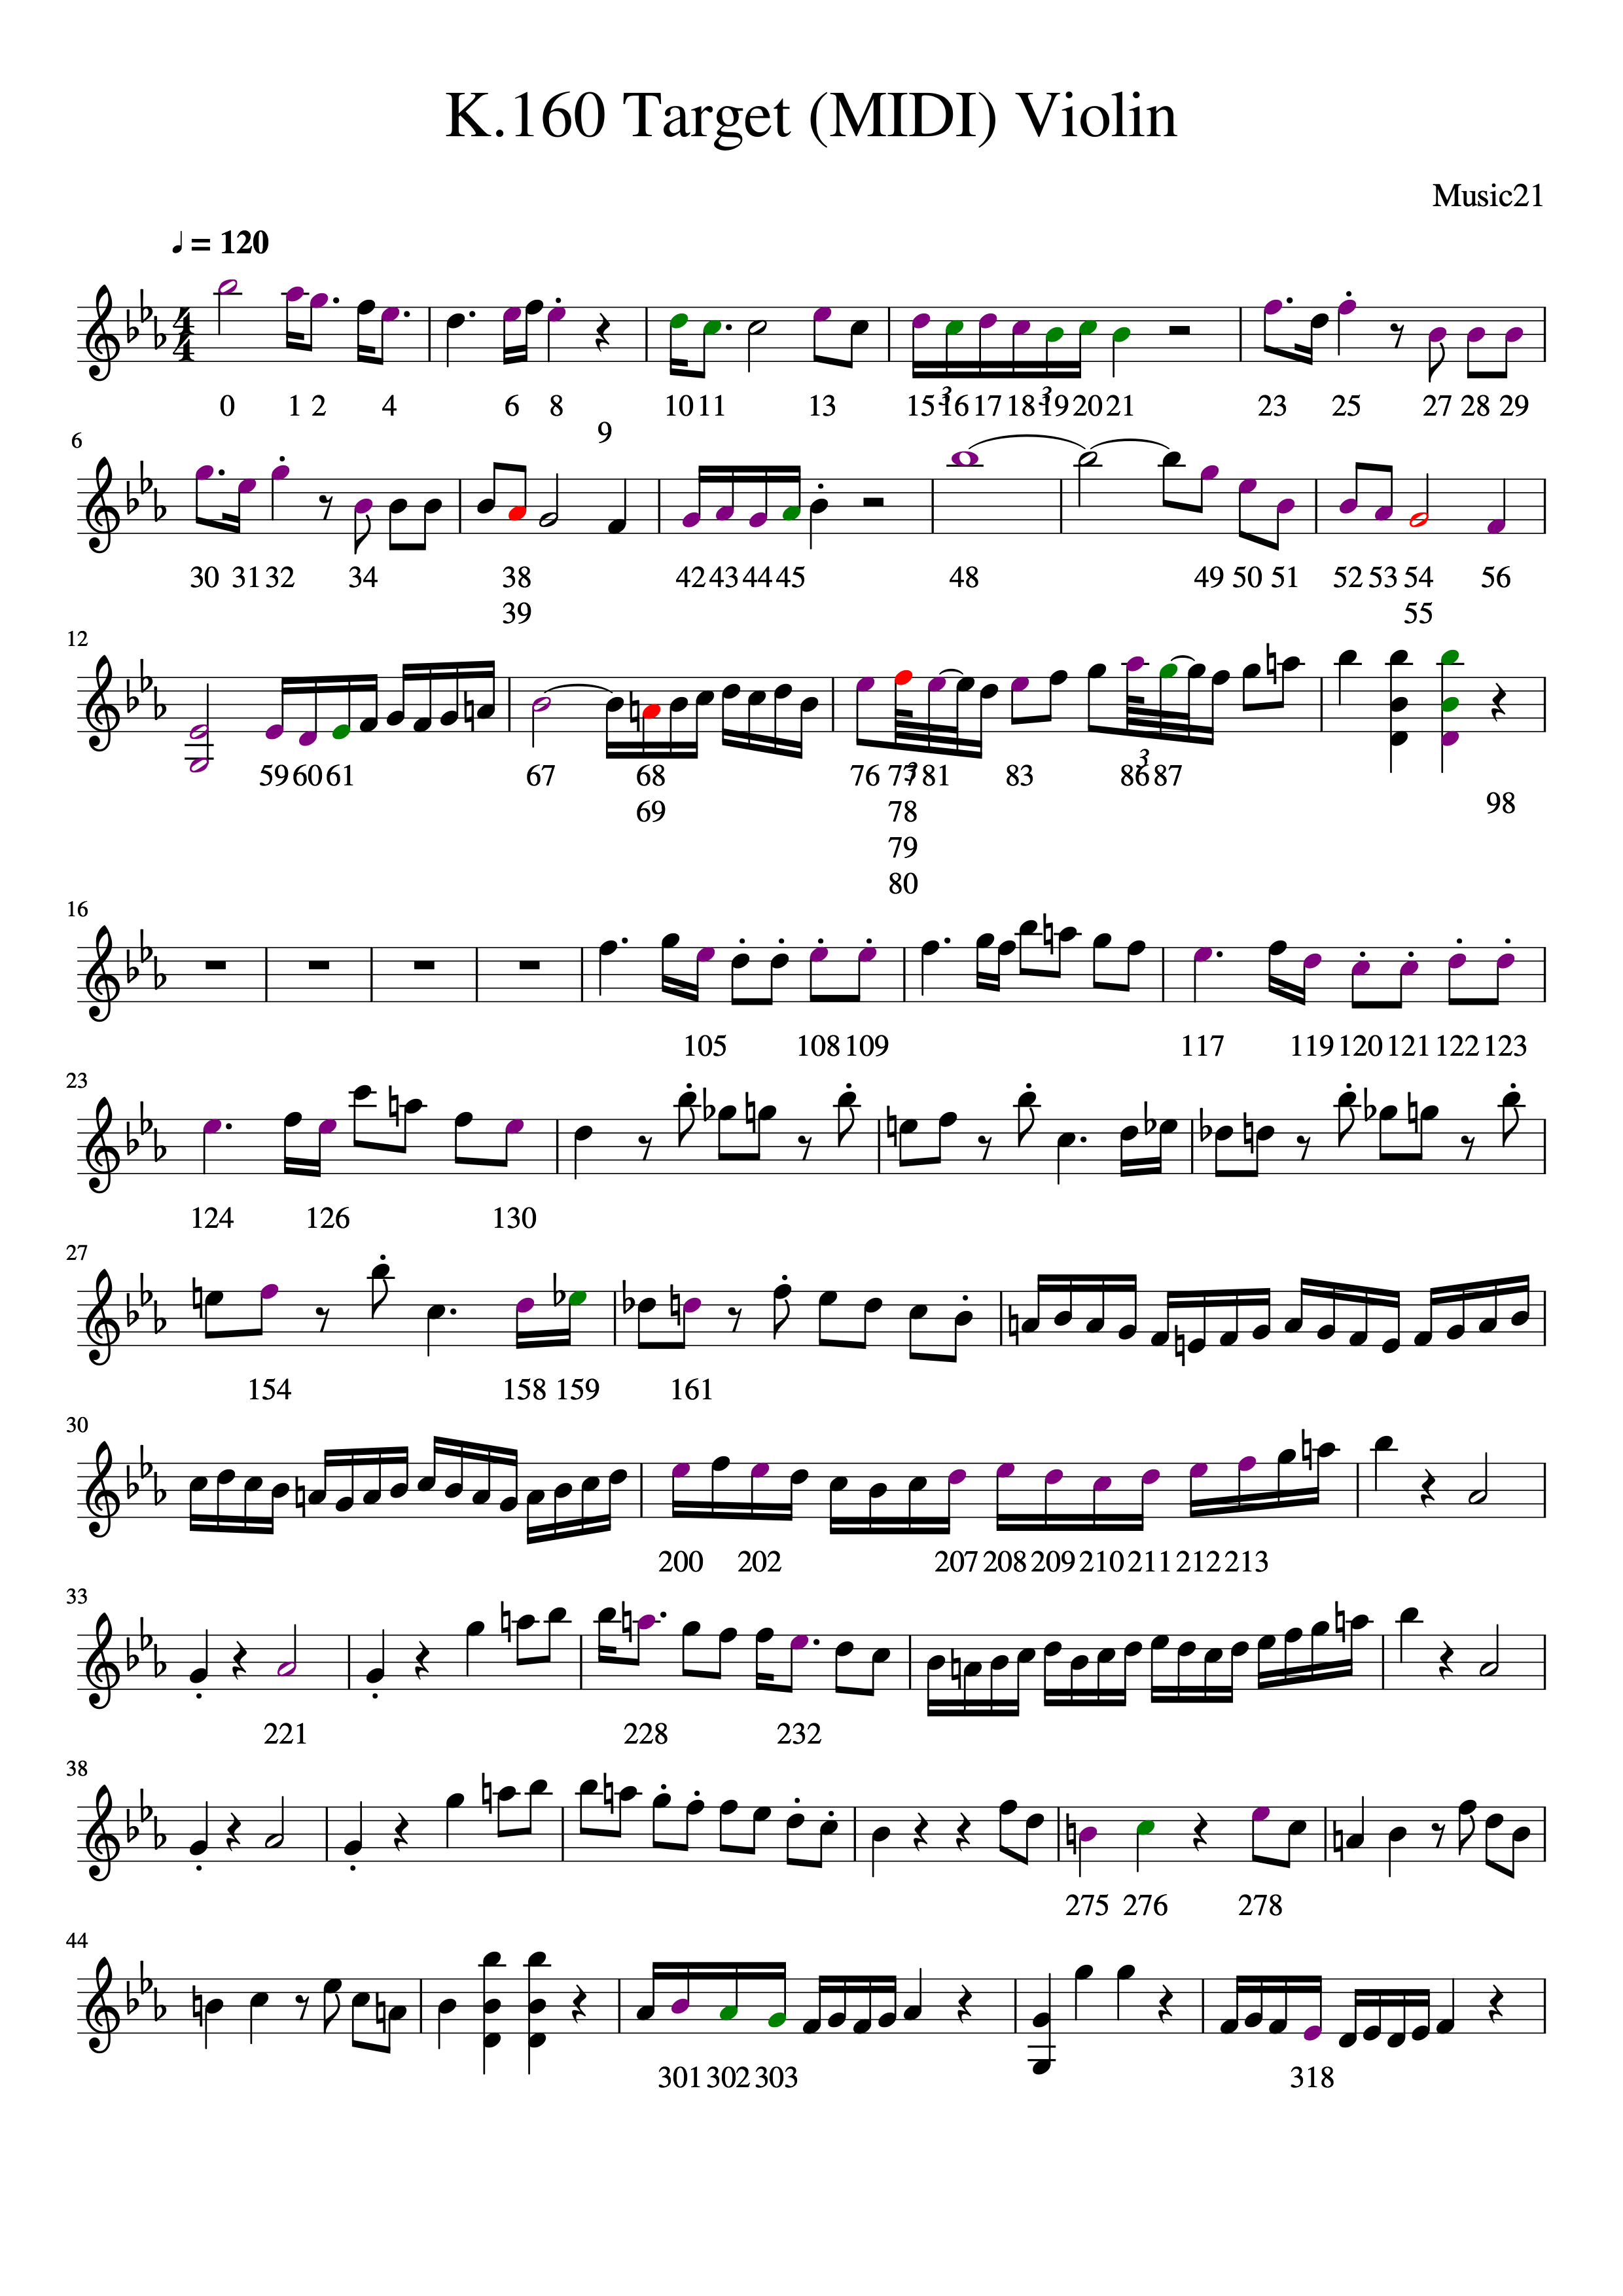
\includegraphics[width =.95\textwidth]{k160postalignv1midi-1}
\caption{Post-alignment visualization of the MIDI Violin 1 part in K.160.}
\end{figure}

\begin{figure}[H]
\centering
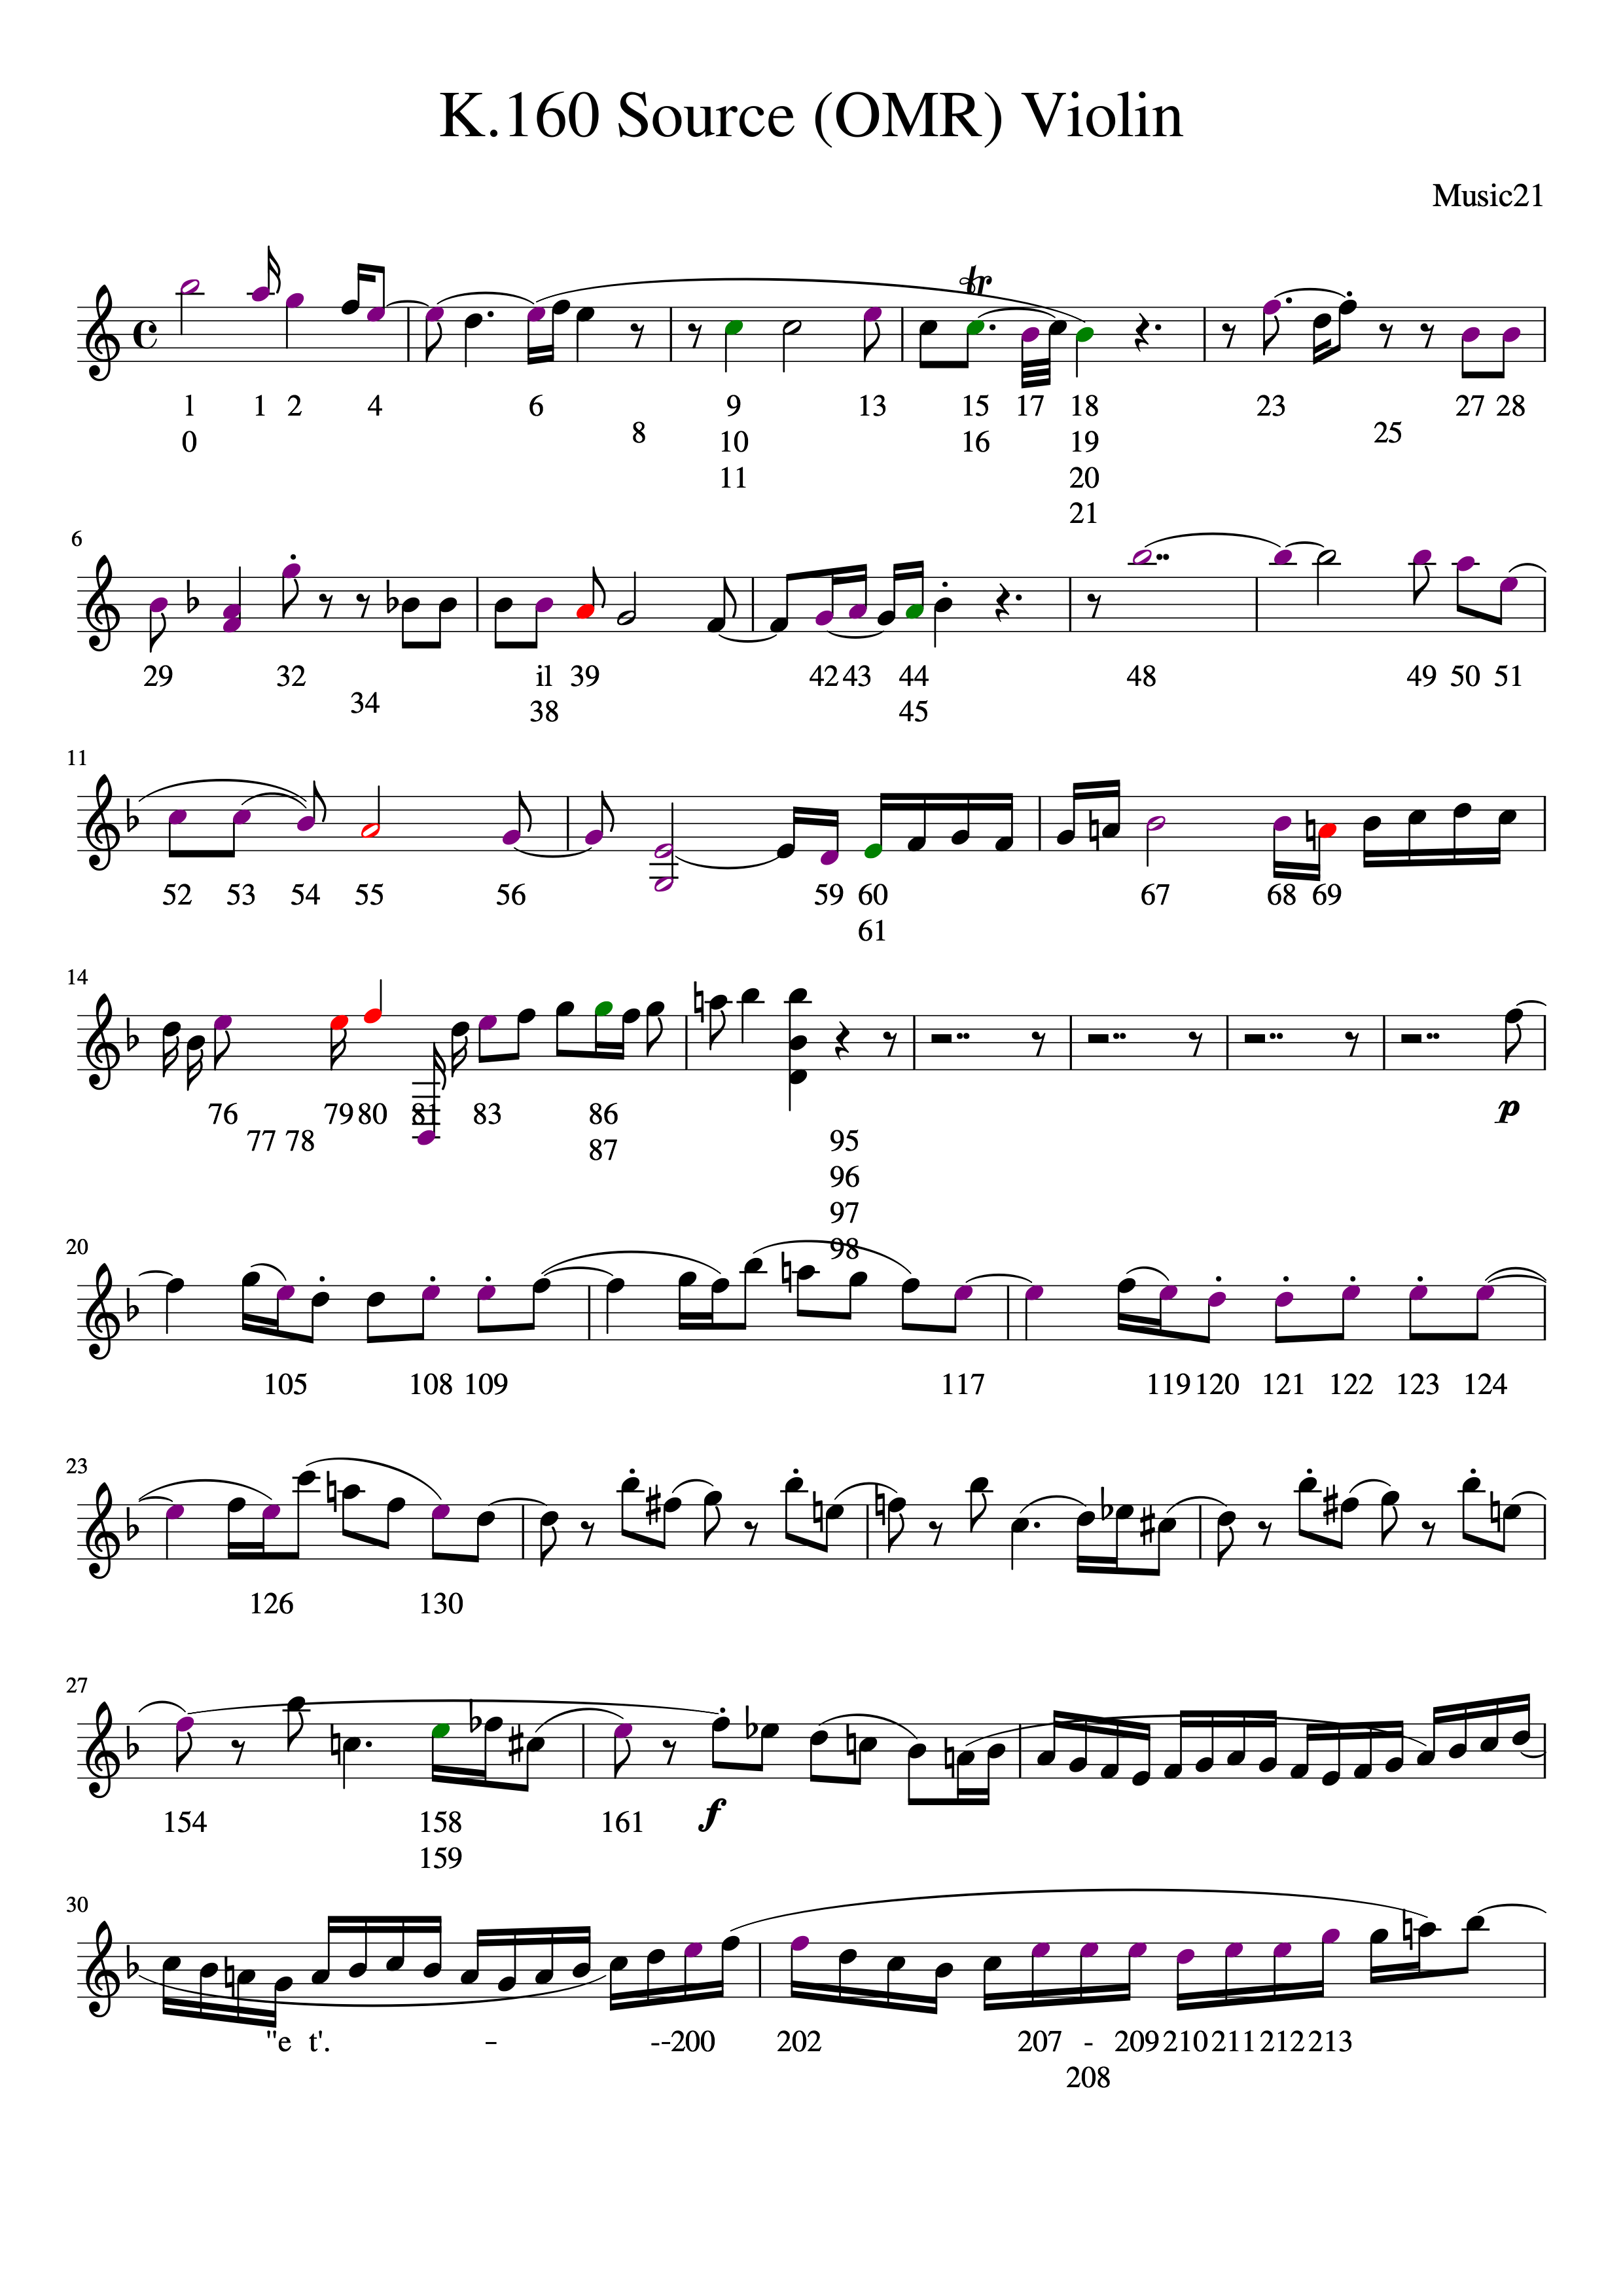
\includegraphics[width =.95\textwidth]{k160postalignv1omr-1}
\caption{Post-alignment visualization of the OMR Violin 1 part in K.160.}
\end{figure}

\begin{figure}[H]
\centering
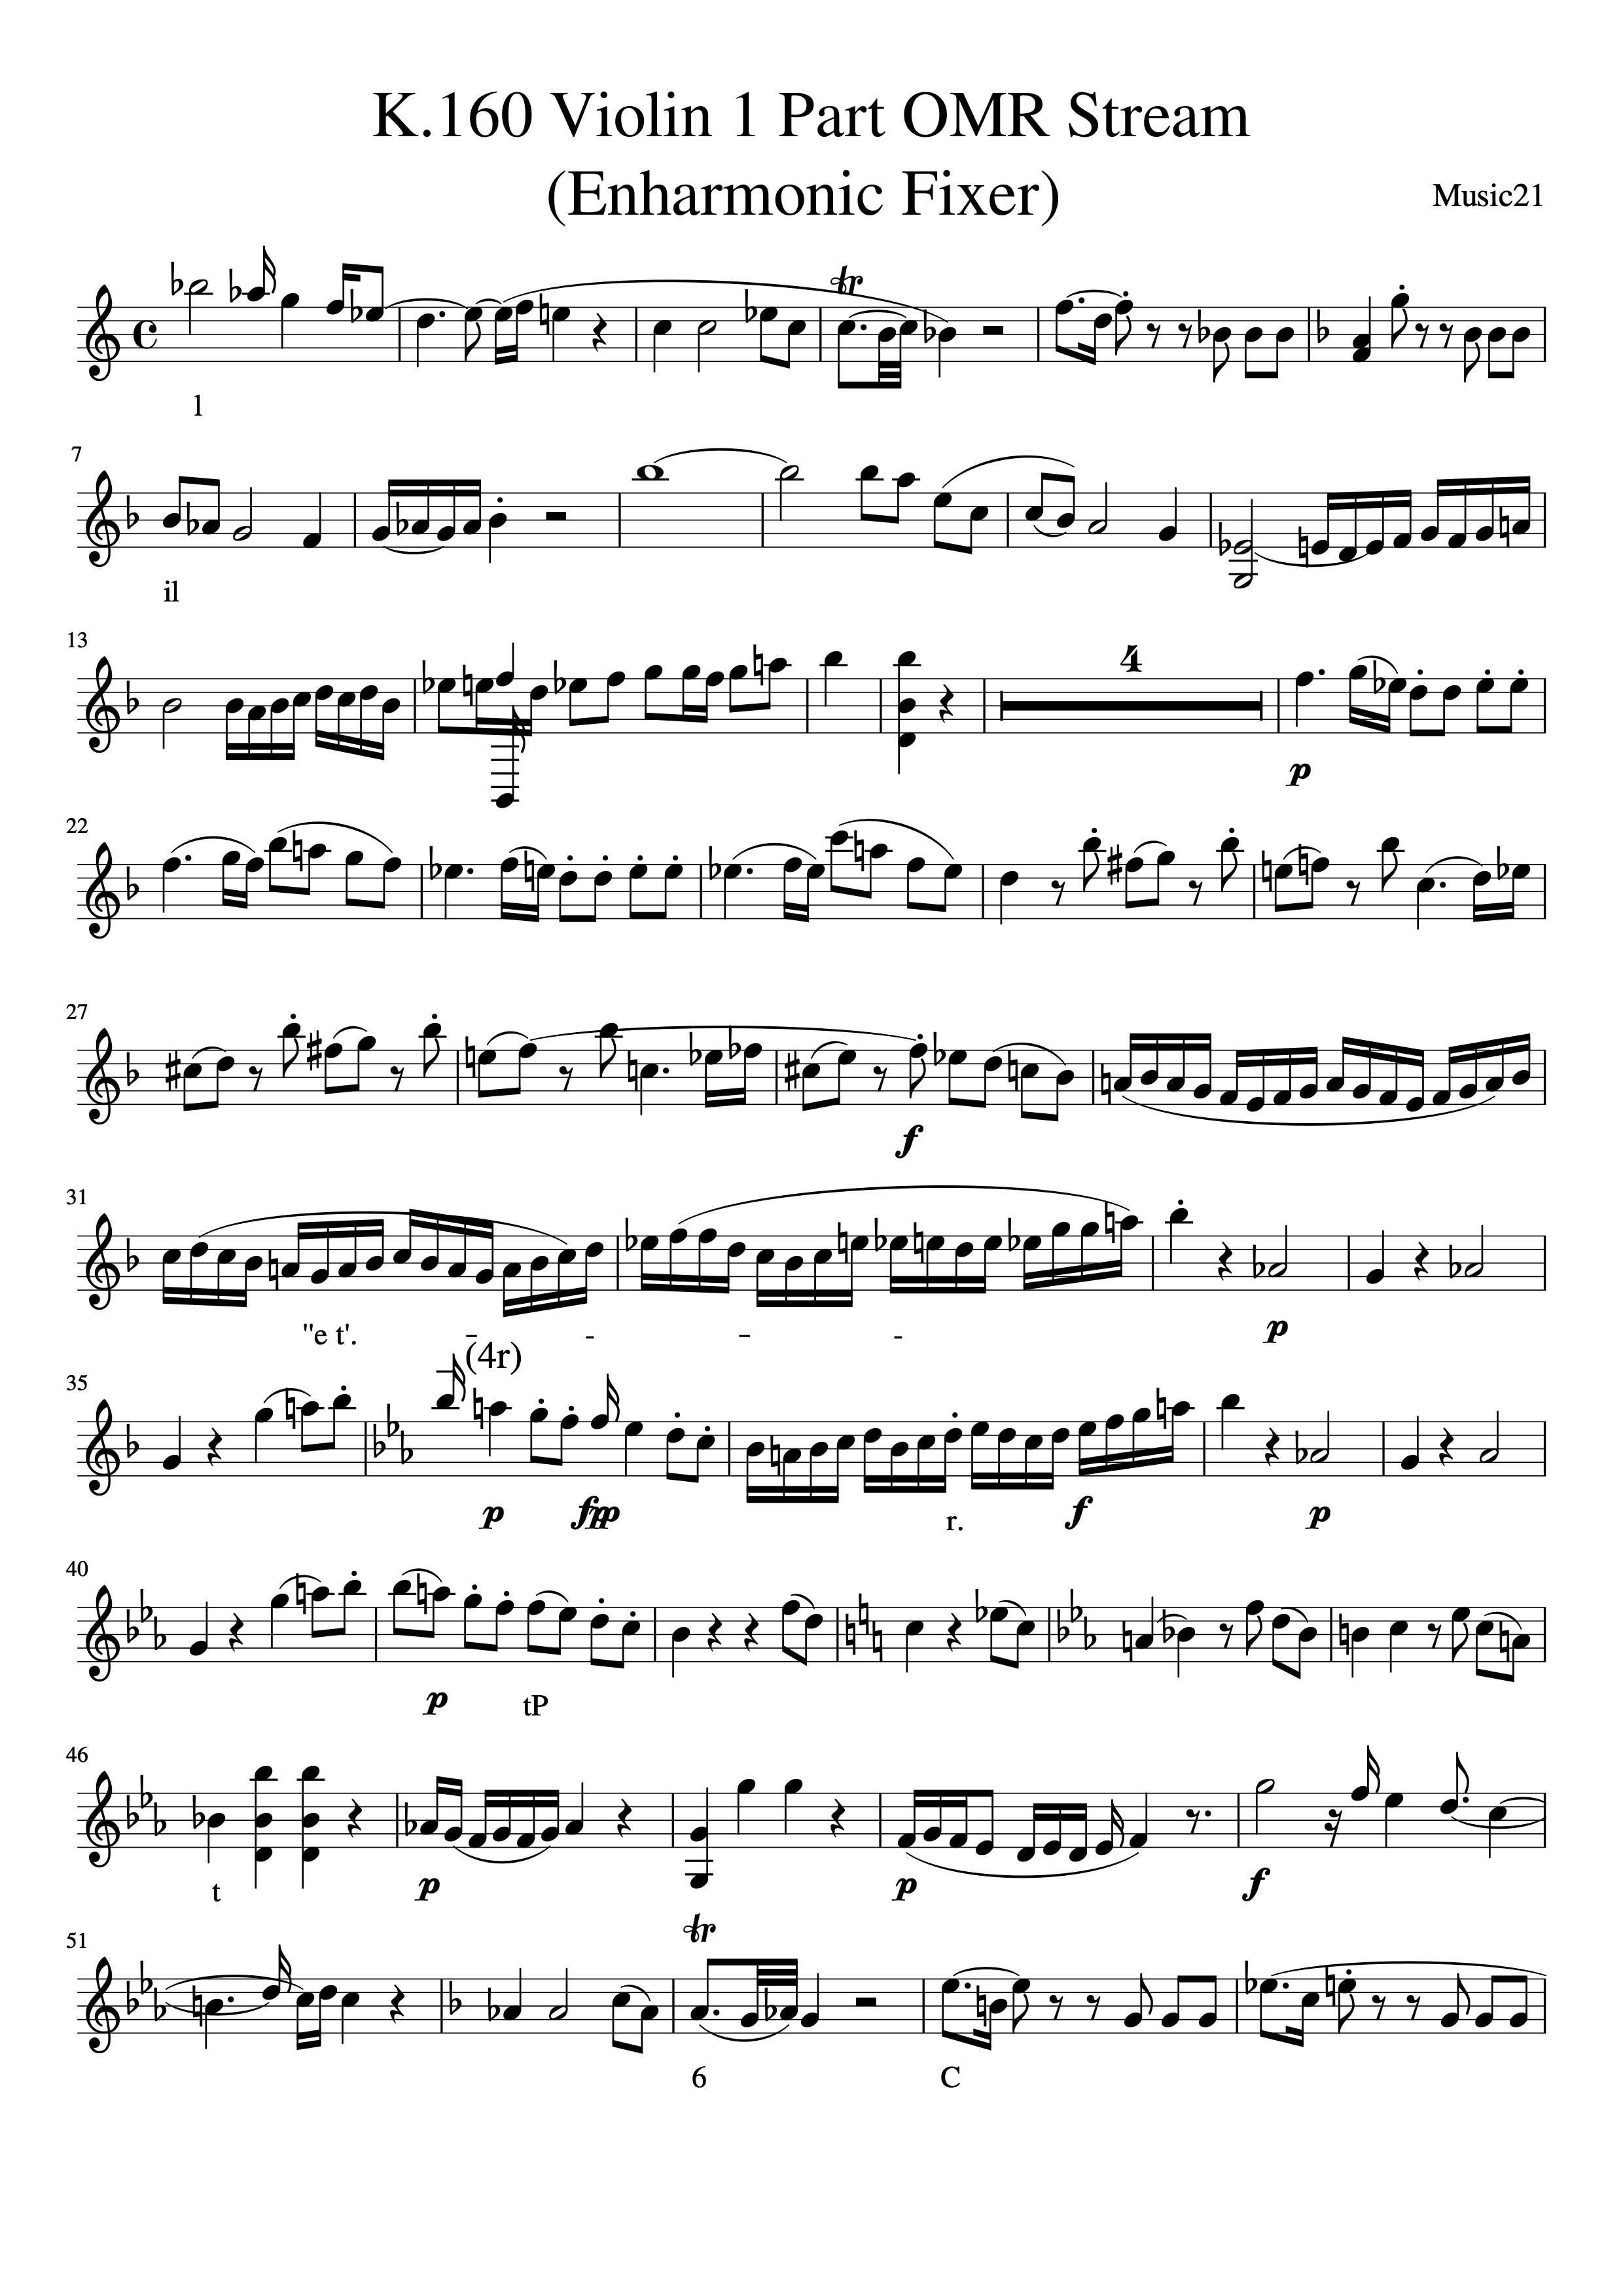
\includegraphics[width =.95\textwidth]{k160postfixv1-1}
\caption{Post-enharmonic and pitch fixing visualization of the OMR Violin 1 part in K.160.}
\end{figure}

\subsection{}
\section{Timing} \label{timing}

